\section{三维连续时间系统:洛伦兹系统}
洛伦兹(Lorenz)系统是1963年由Edward Lorenz提出的描述空气流体运动的一个数学模型。1998年,S.Smale提出21世纪的18个著名的数学问题,其中第14个问题就是关于洛伦兹系统的研究。迄今为止,对洛伦兹系统的研究无论是从数学、物理还是工程上都是十分重要的问题。

\subsection{洛伦兹系统的动力学}
洛伦兹系统的动力学方程表示为:
\begin{equation}
    \begin{cases}
        \dot{x}=\sigma(y-x)\\
        \dot{y}=x(\rho-z)-y\\
        \dot{z}=xy-\beta z
    \end{cases}\
\end{equation}

该方程描述了一个三维相空间的三个分量对时间的变化率。其中$x$代表对流强度,$y$代表上升流和下降流的温差,$z$代表铅直方向温度分布的非线性强度。$c$是Rayleigh数,为系统的主要控制参数,$a$是Prandt数,$b$是外形比。Lorenz系统具有非线性、非周期性和确定性的性质。参数$\sigma$,$\rho$,$\beta$取不同值时Lorenz系统表现出不同的动力学行为。如在$\rho<1$时,系统只有一个不动点,即原点,所有轨道的长期行为都趋于原点;当$\rho=1$时系统发生了叉式分岔,在$\rho>1$时出现了两个不动点,不动点的稳定性可由其他参数满足的条件确定。三个不动点的坐标分别为$(0,0,0)$、$(\sqrt{\beta(\rho-1)},\sqrt{\beta(\rho-1)},\rho-1)$、$(-\sqrt{\beta(\rho-1)},-\sqrt{\beta(\rho-1)},\rho-1)$。当我们将三个参数取一组特定的值$\rho=28$,$\sigma=10$,$\beta=8/3$时,Lorenz方程的解是混沌的,相空间会存在两个奇异吸引子。

洛伦兹系统的这种动力学特征用传统的非线性动力学知识是比较难分析的,其相图如下:
\begin{figure}
	\centering
	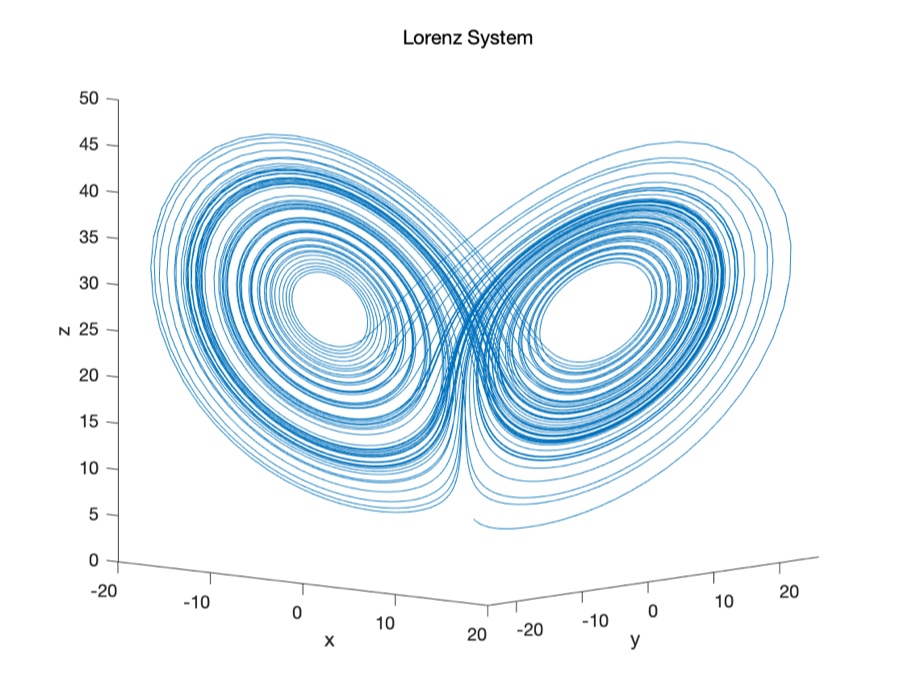
\includegraphics[scale=0.8]{lorenz_phase.png}
    \caption{洛伦兹系统的相图($\rho=28$,$\sigma=10$,$\beta=8/3$)}
    \label{fig:lorz_phas}
\end{figure}
在洛伦兹系统中,所有的非平衡解最终趋向同一个复杂的集合,这就是所谓的洛伦兹吸引子。我们将在取上述参数的条件下,通过Lorenz微分方程演化出相空间的一条轨道,作为Koopman分析的源数据,以此来分析Lorenz系统的特征。

\subsection{洛伦兹系统的Koopman算符本征函数}
\subsubsection{正交完备基函数空间}
\begin{figure}
    \centering
    \subfloat[实部]{
      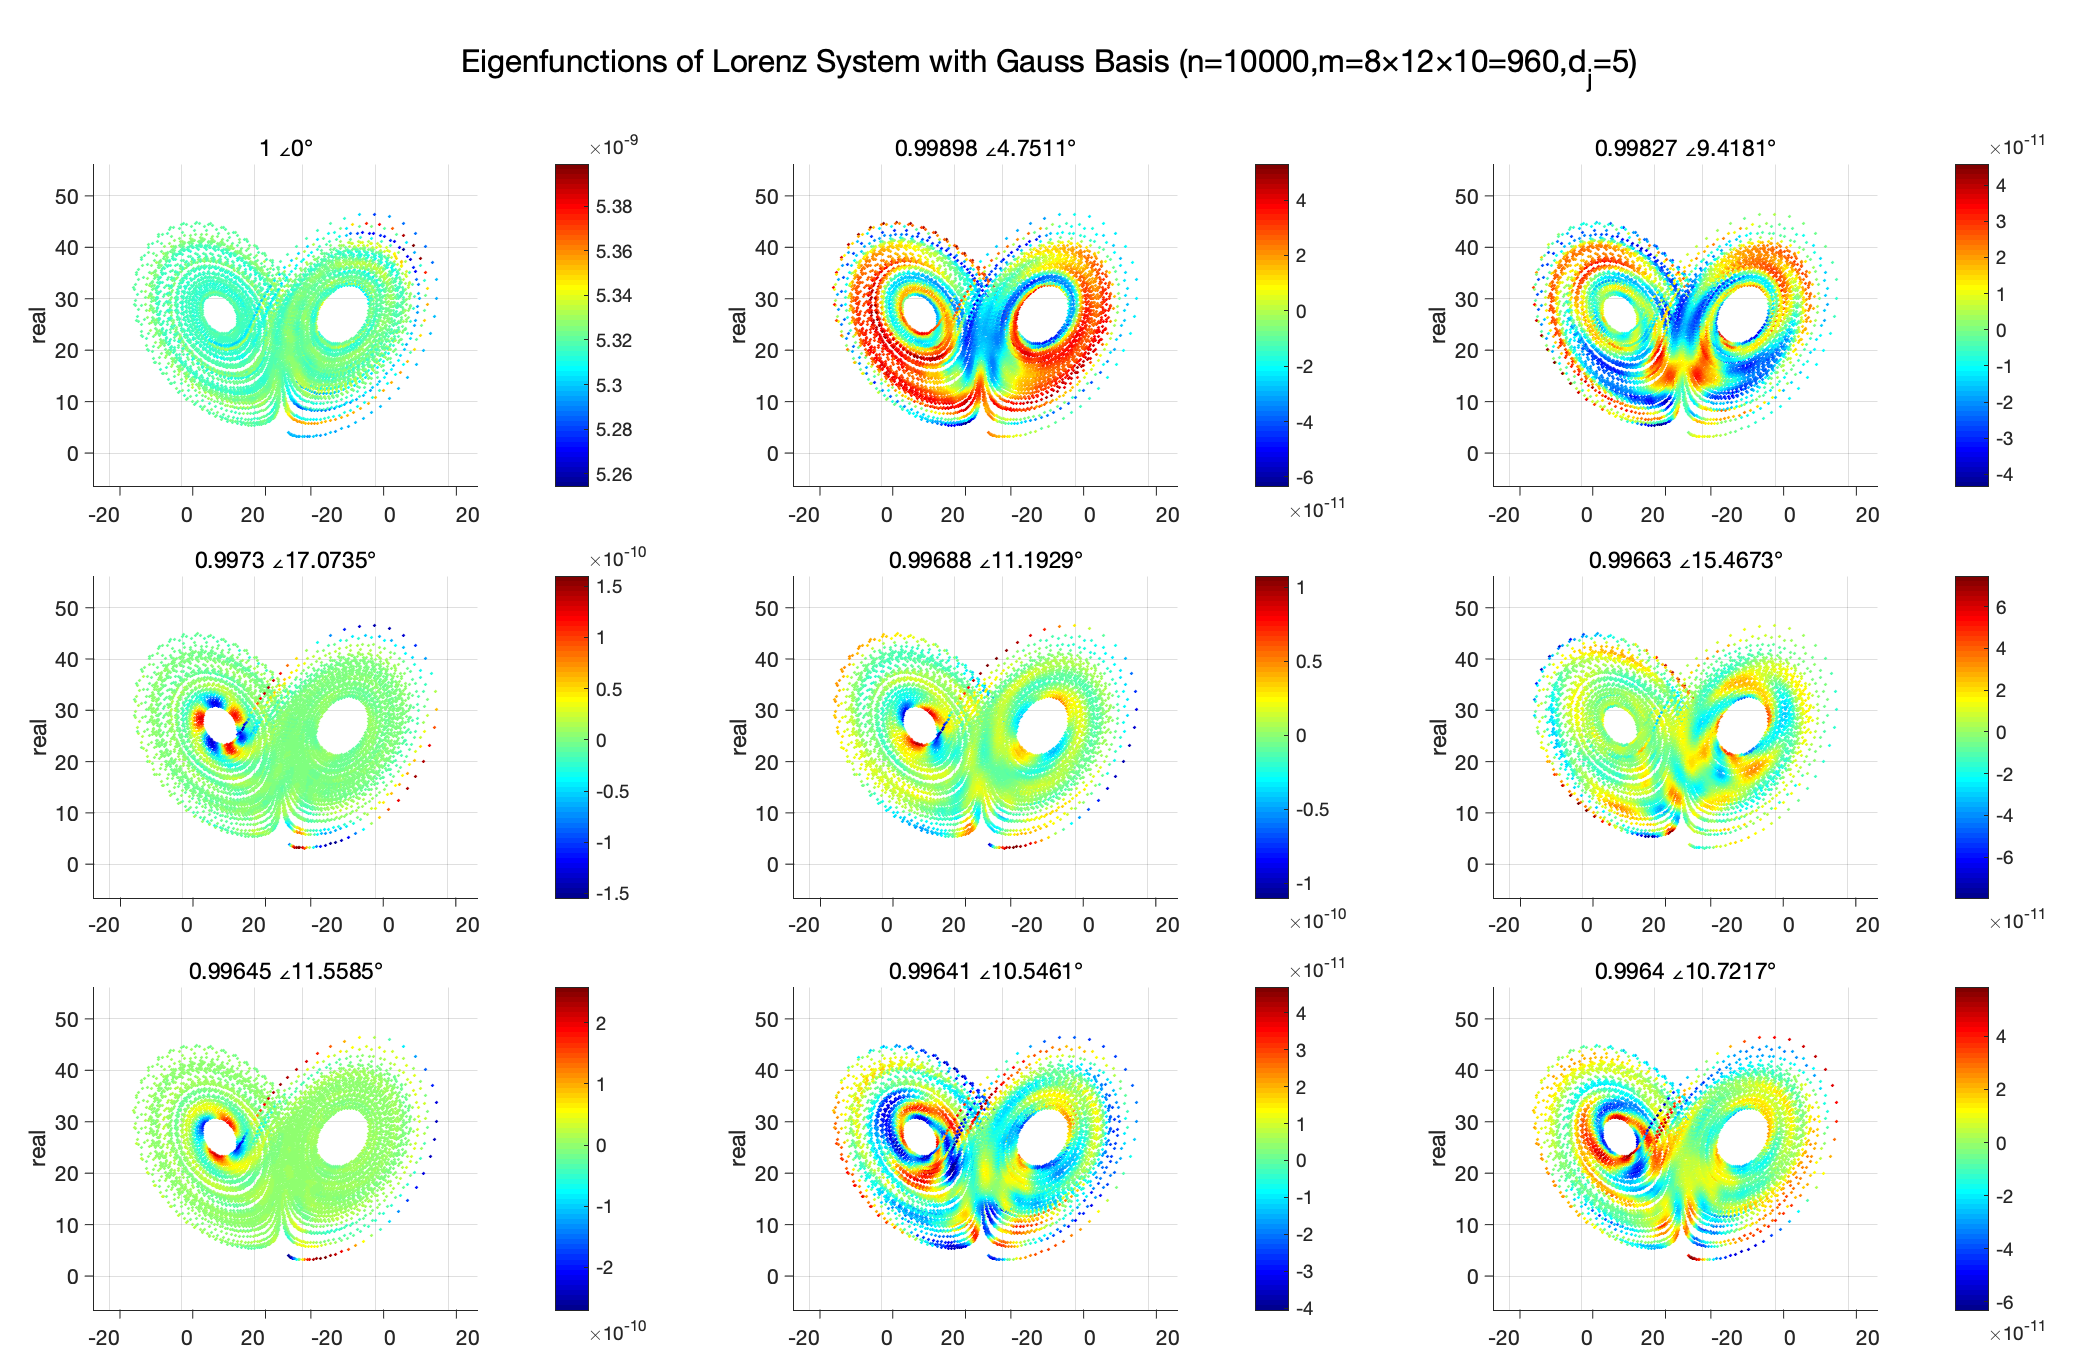
\includegraphics[scale=0.2]{lorenz/Lorenz_eigen_Gauss_leftU_real_n10000m960}}
    \subfloat[虚部]{
      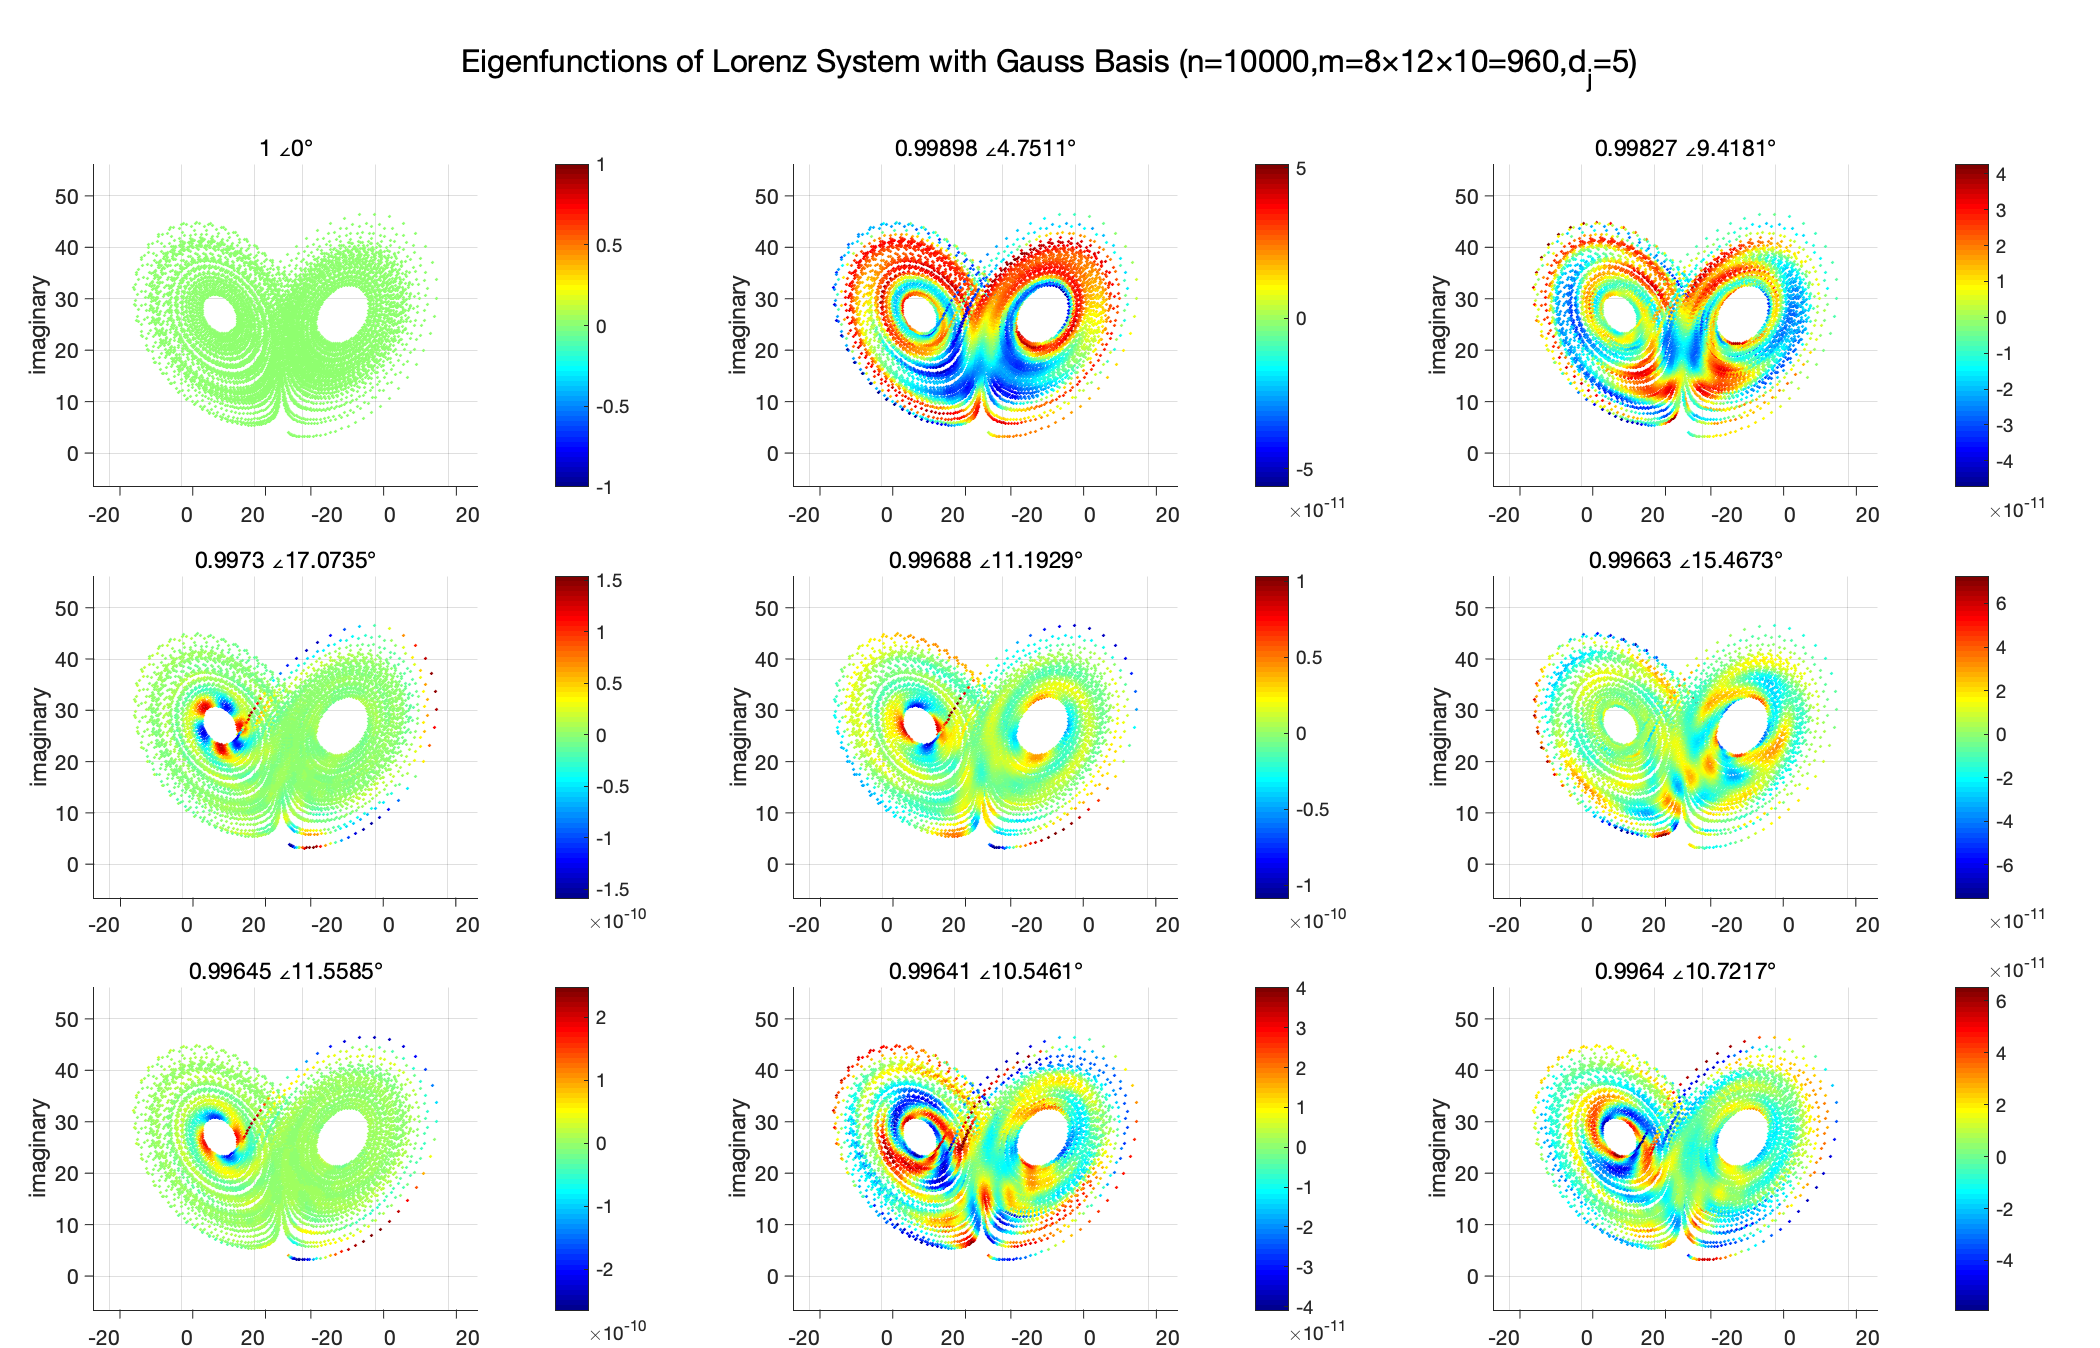
\includegraphics[scale=0.2]{lorenz/Lorenz_eigen_Gauss_leftU_imag_n10000m960}}
    \\
    \subfloat[模]{
      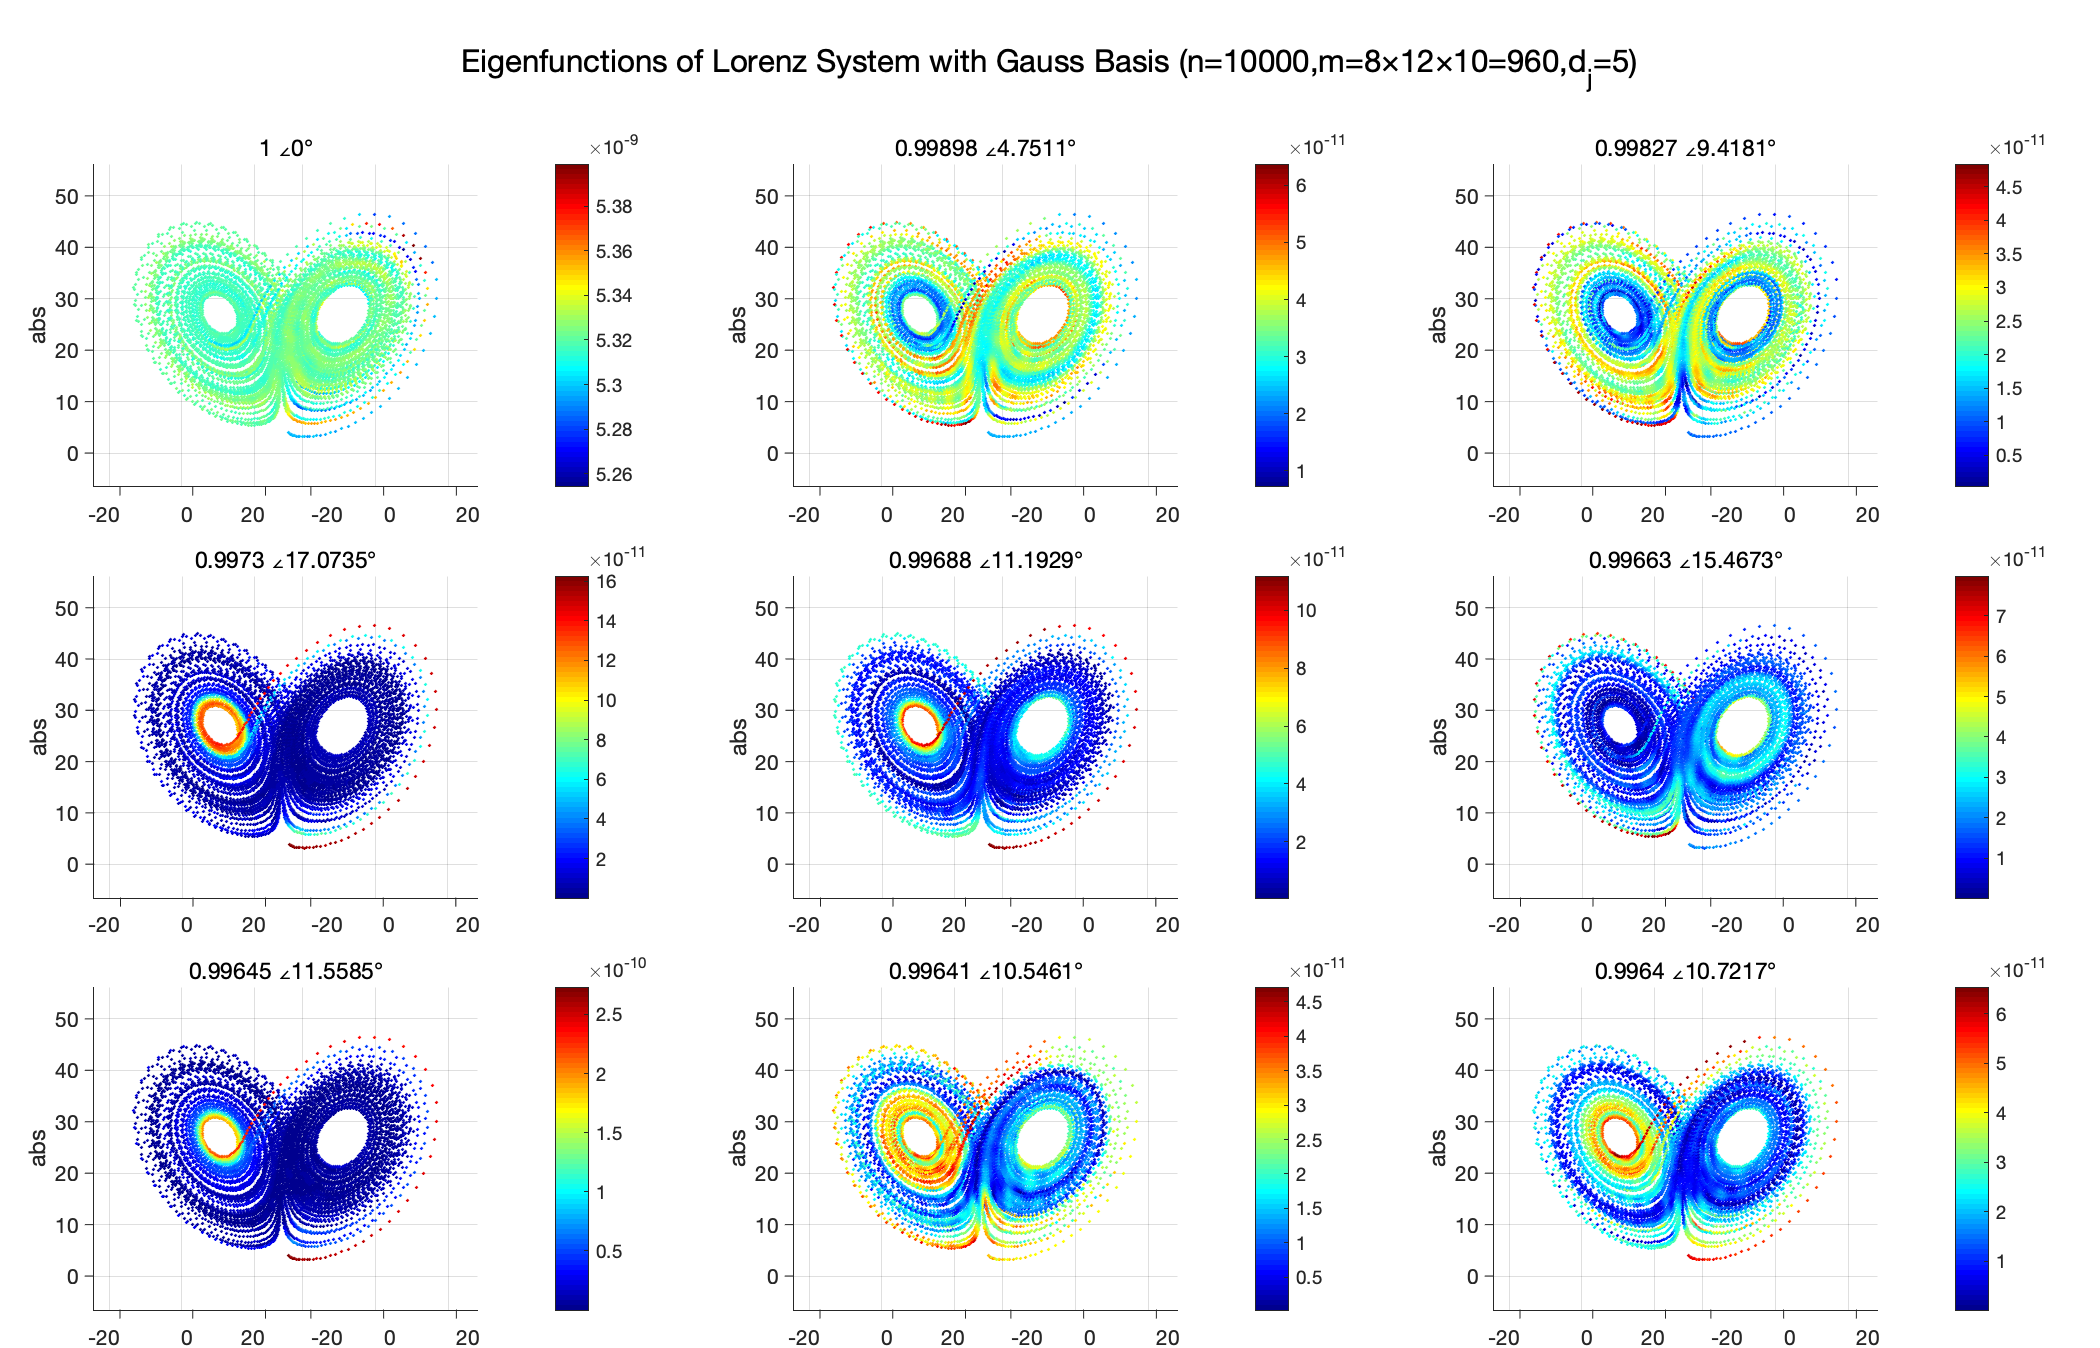
\includegraphics[scale=0.2]{lorenz/Lorenz_eigen_Gauss_leftU_abs_n10000m960}}
    \subfloat[幅角]{
      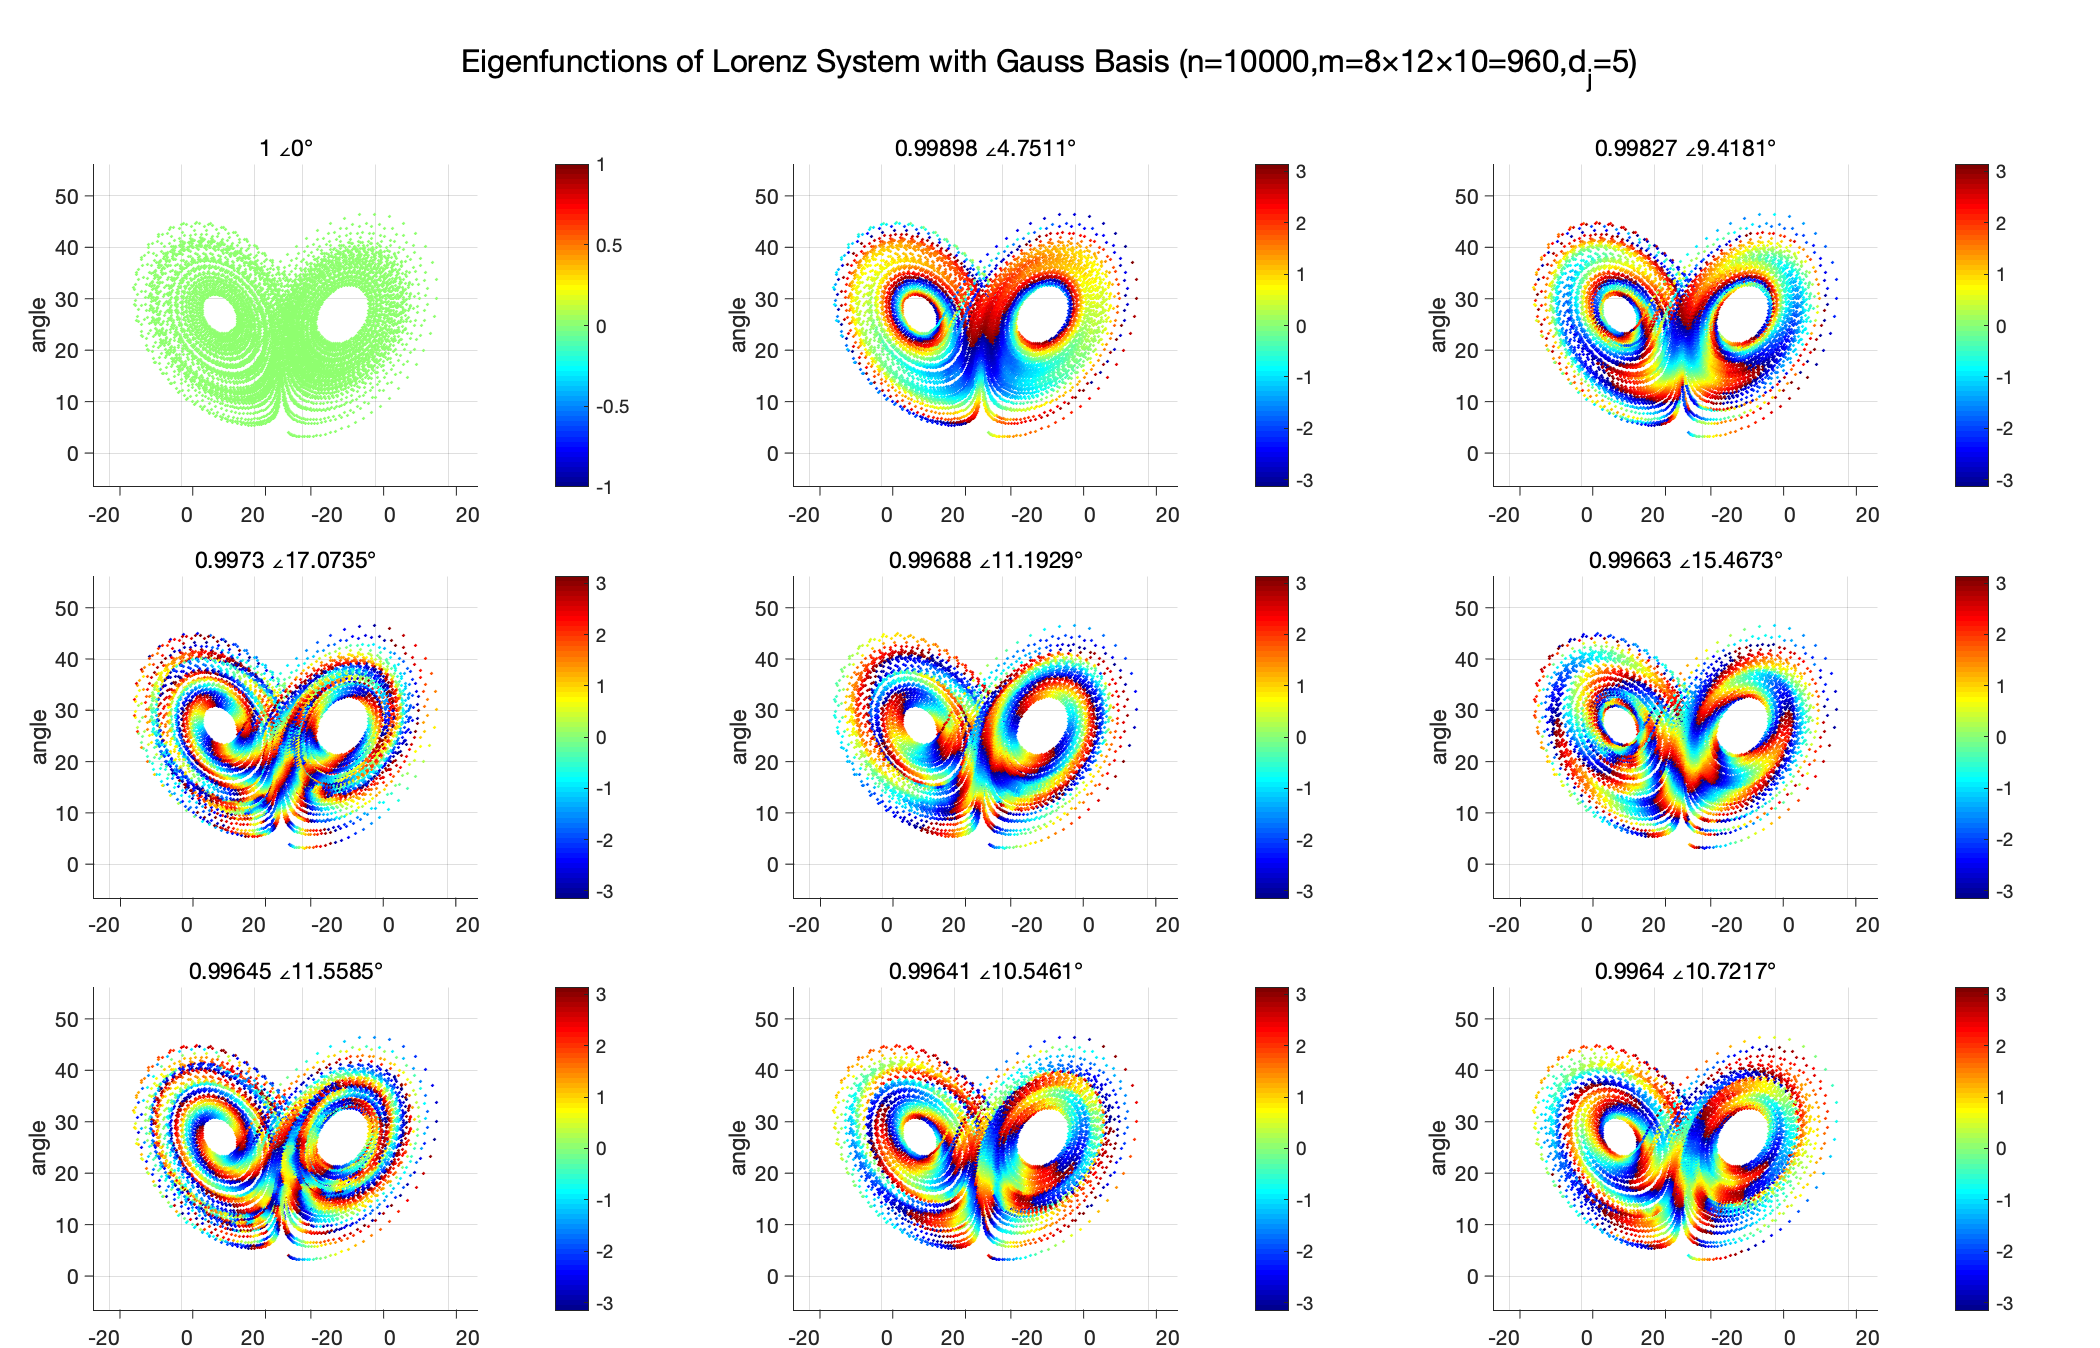
\includegraphics[scale=0.2]{lorenz/Lorenz_eigen_Gauss_leftU_angle_n10000m960}}
    \\
    \caption{洛伦兹系统三维高斯基的本征函数($n=10000,m=960$)}
\end{figure}

\begin{figure}
	\centering
	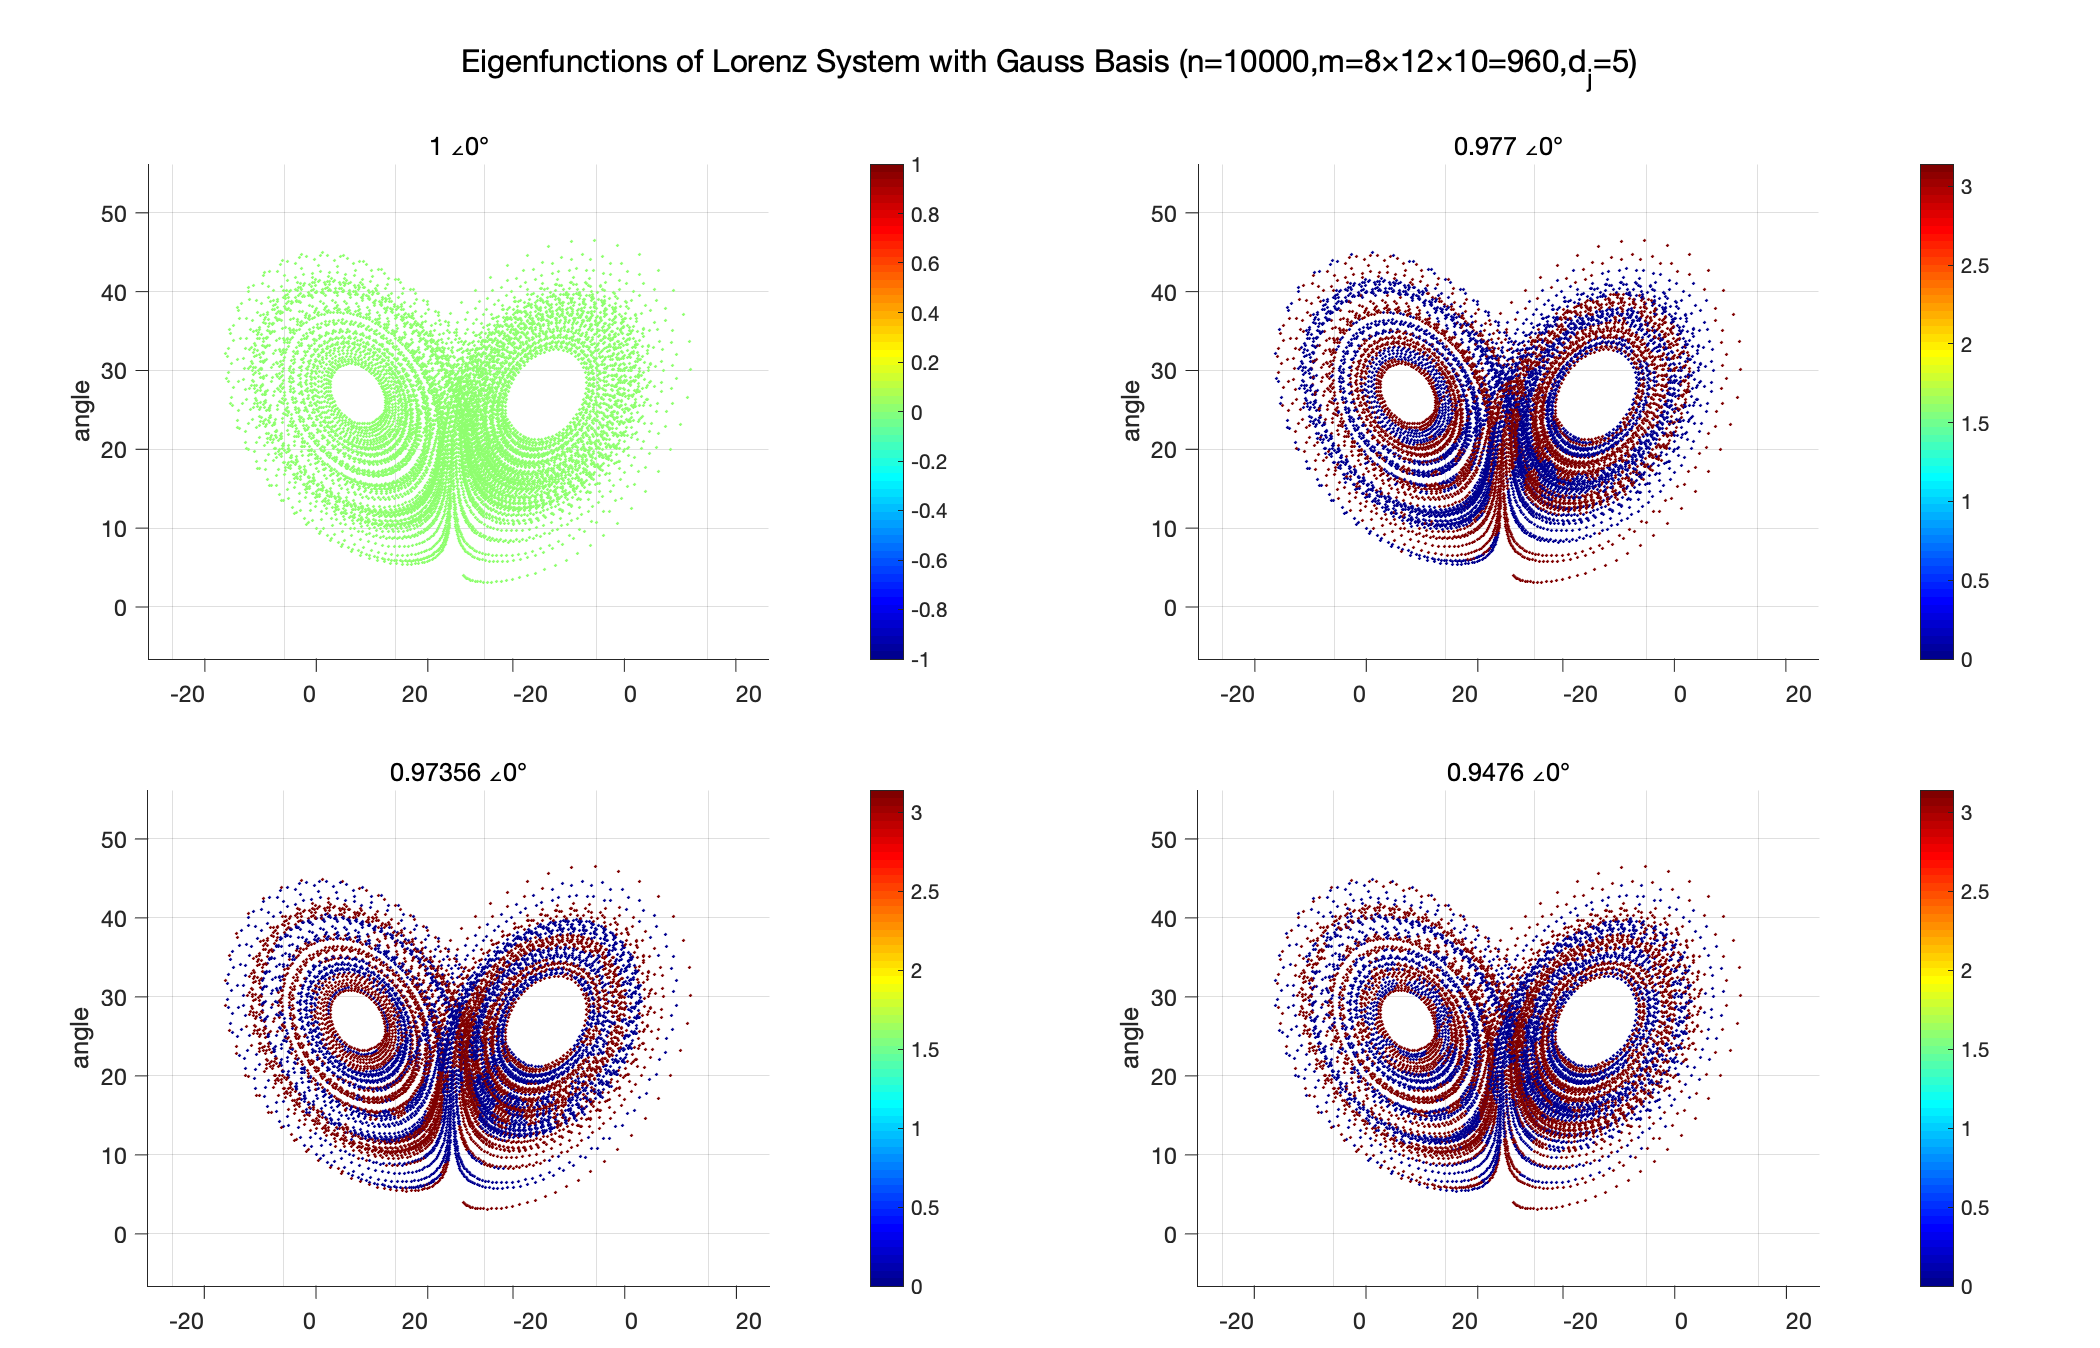
\includegraphics[scale=0.4]{lorenz/Lorenz_eigen_Gauss_leftU_realL_n10000m960}
    \caption{洛伦兹系统三维高斯基的本征函数(幅角)($n=10000,m=960$)}
\end{figure}

\subsubsection{自然基函数空间}
\begin{figure}
    \centering
    \subfloat{
      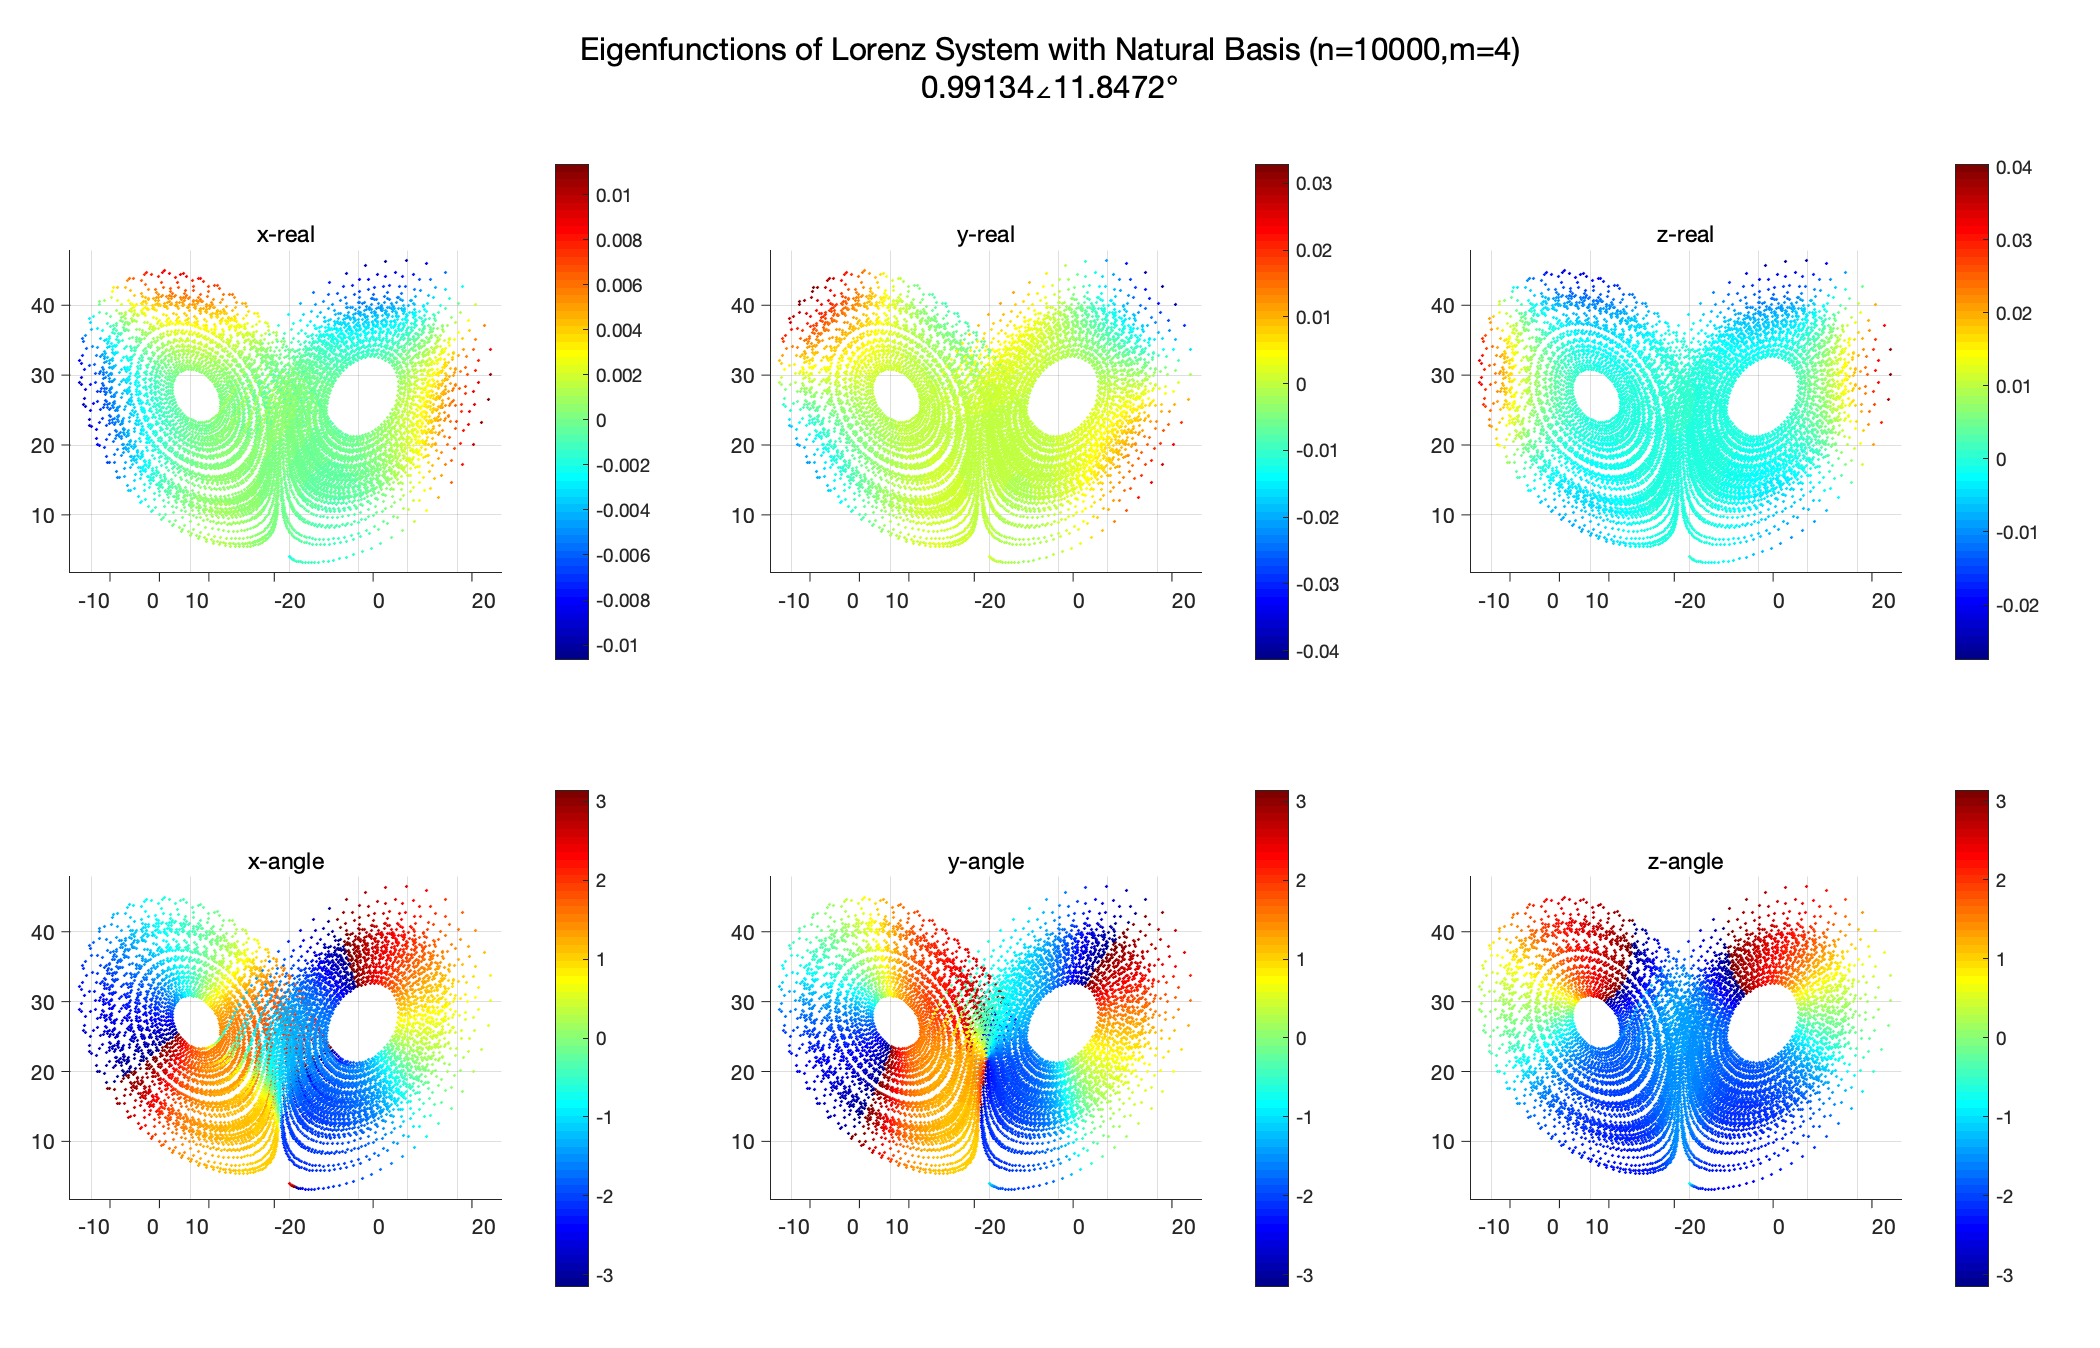
\includegraphics[scale=0.2]{lorenz/natural/Lorenz_eigen_natural_n10000m4figure1}}
    \subfloat{
      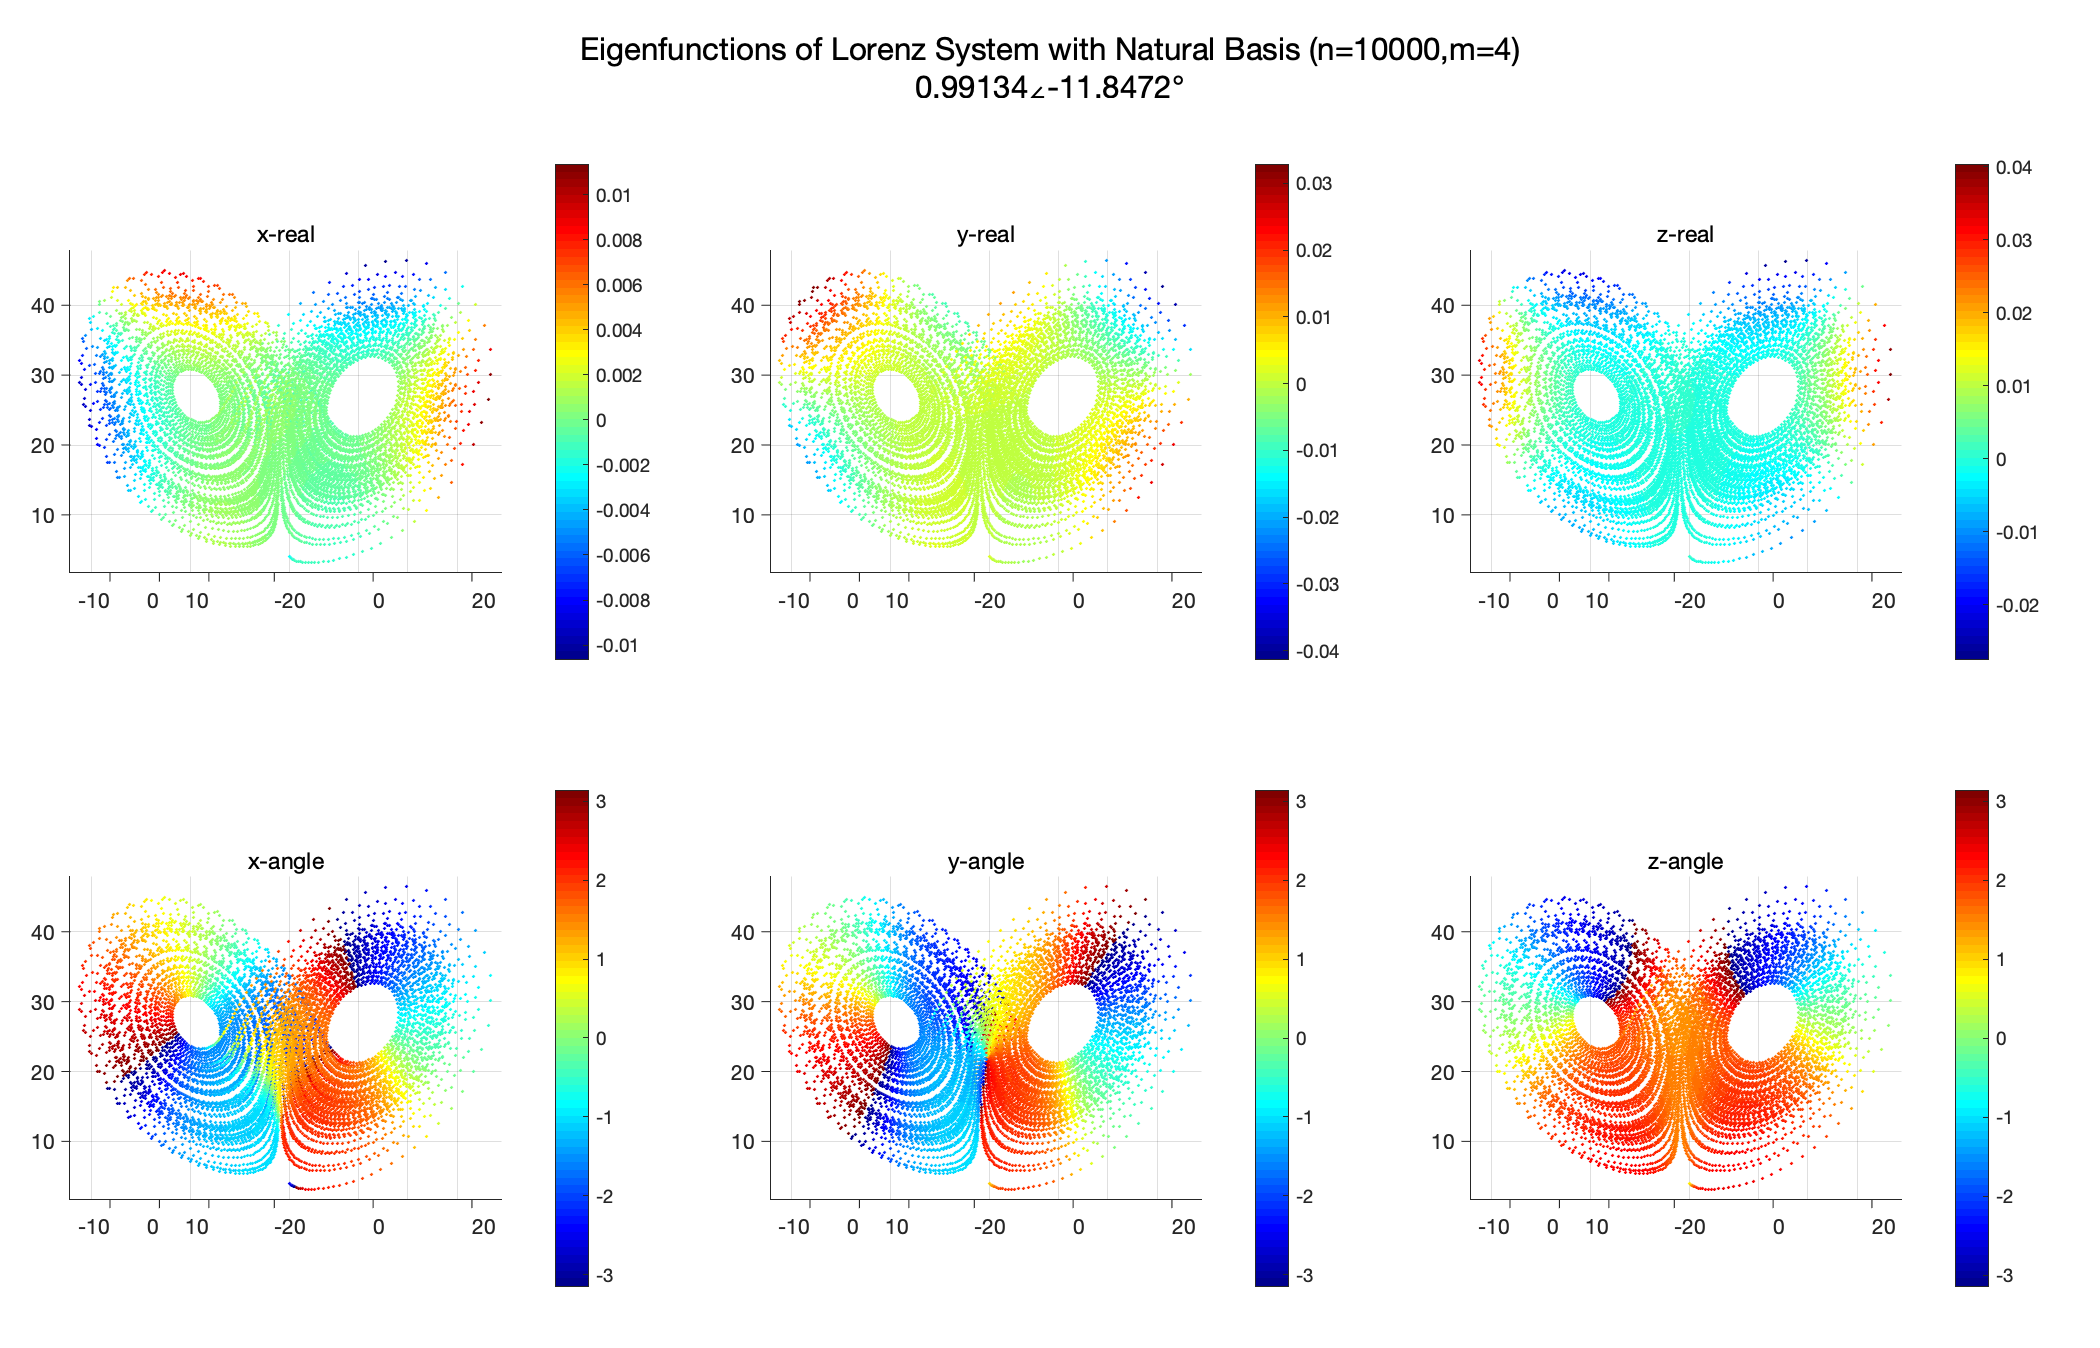
\includegraphics[scale=0.2]{lorenz/natural/Lorenz_eigen_natural_n10000m4figure2}}
    \\
    \subfloat{
      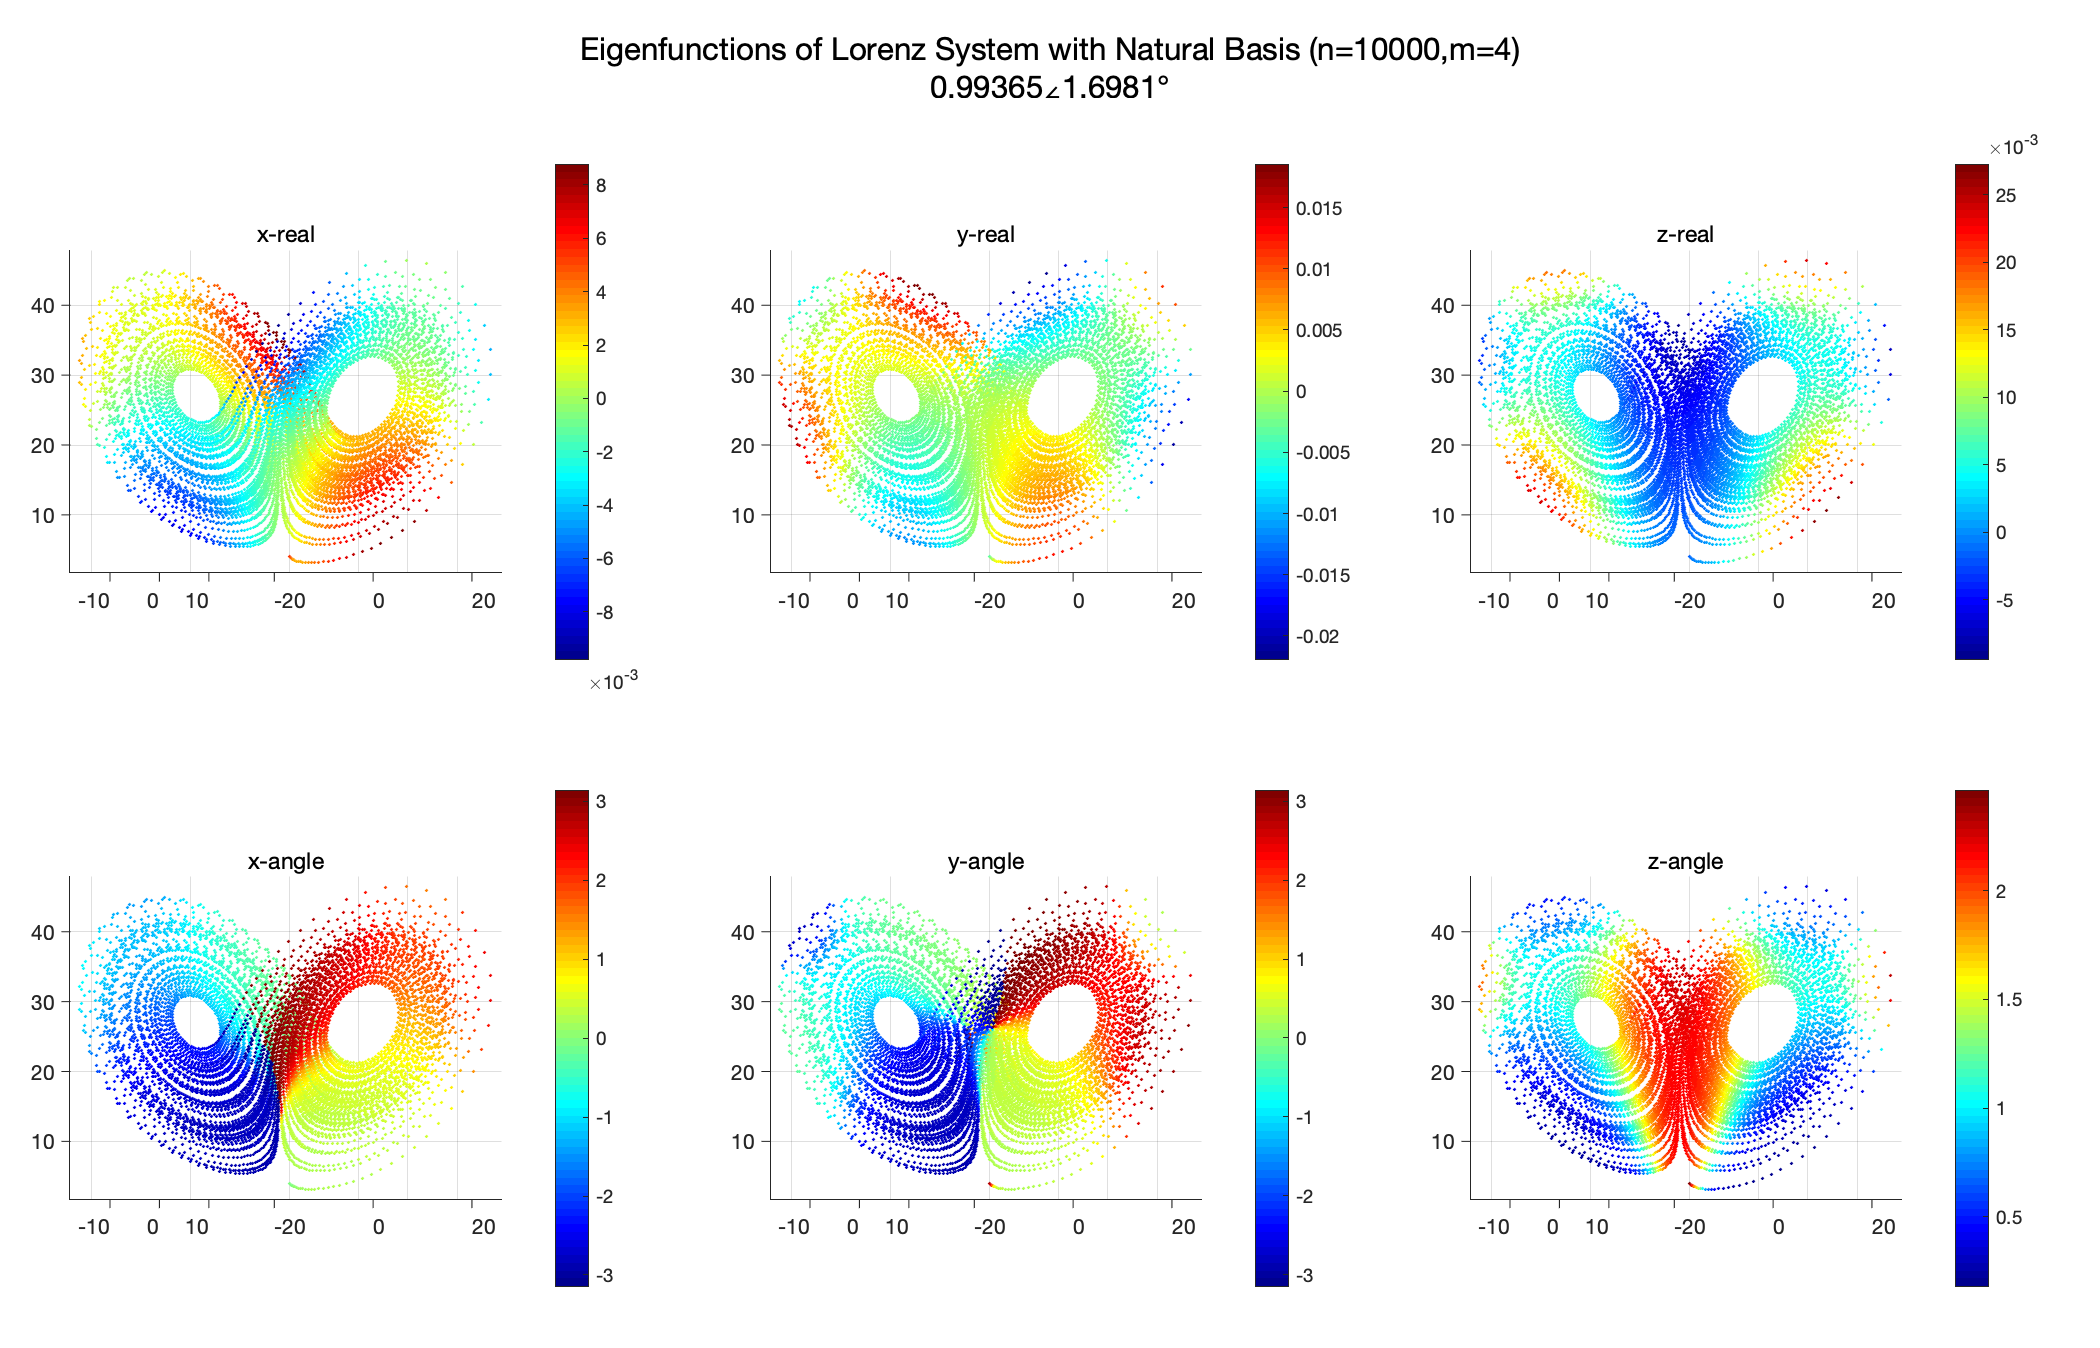
\includegraphics[scale=0.2]{lorenz/natural/Lorenz_eigen_natural_n10000m4figure3}}
    \subfloat{
      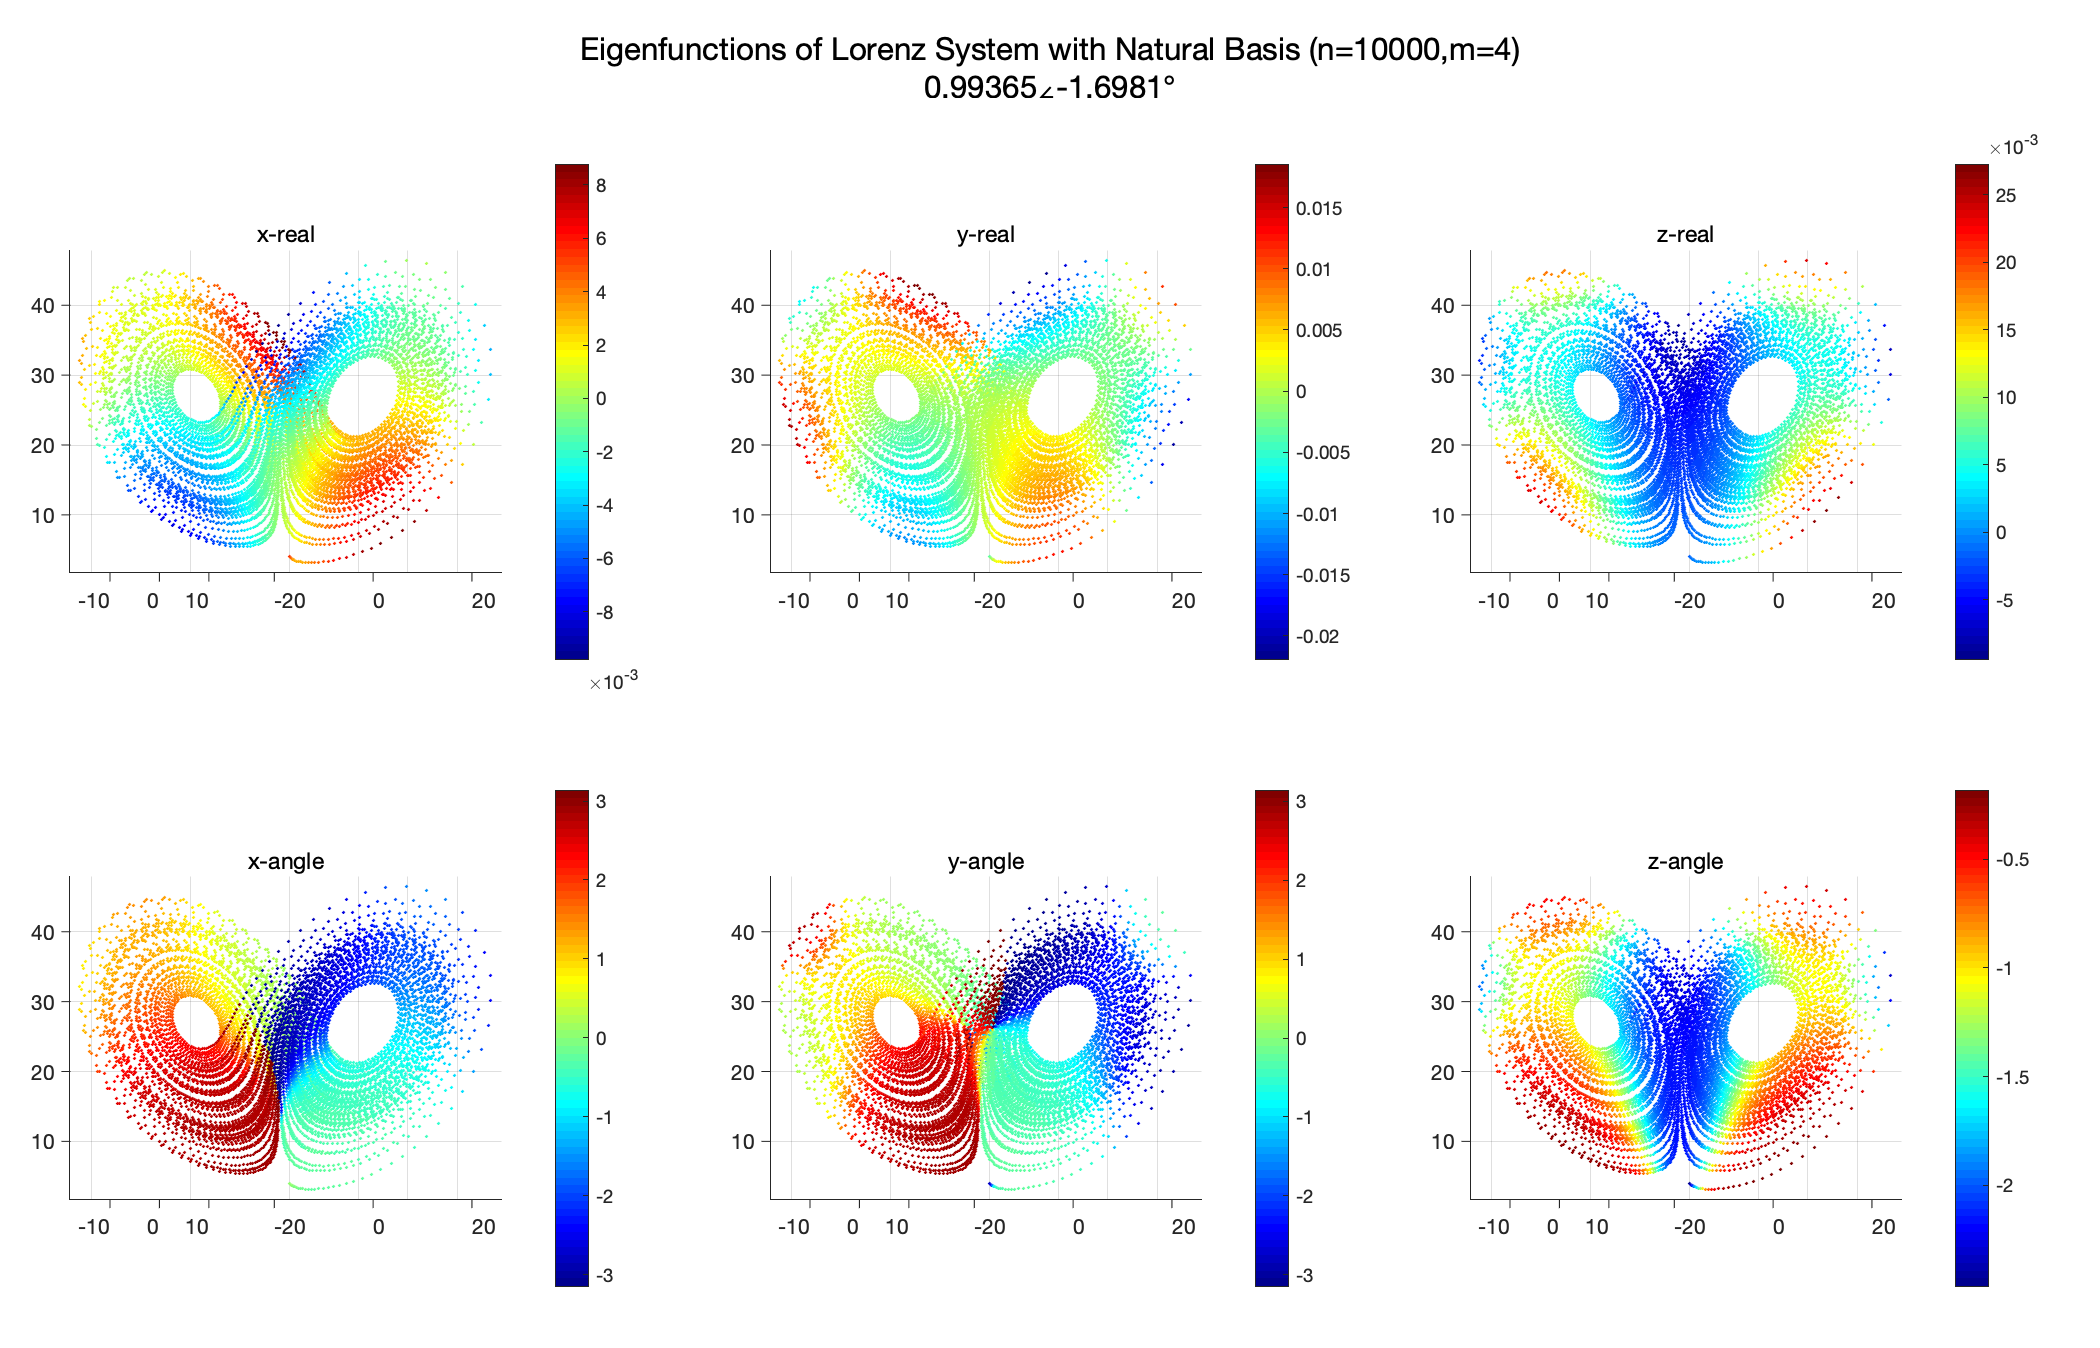
\includegraphics[scale=0.2]{lorenz/natural/Lorenz_eigen_natural_n10000m4figure4}}
    \\
    \caption{洛伦兹系统自然基下的本征函数($n=10000,m=4$)}
\end{figure}

\begin{figure}
    \centering
    \subfloat[m=1]{
      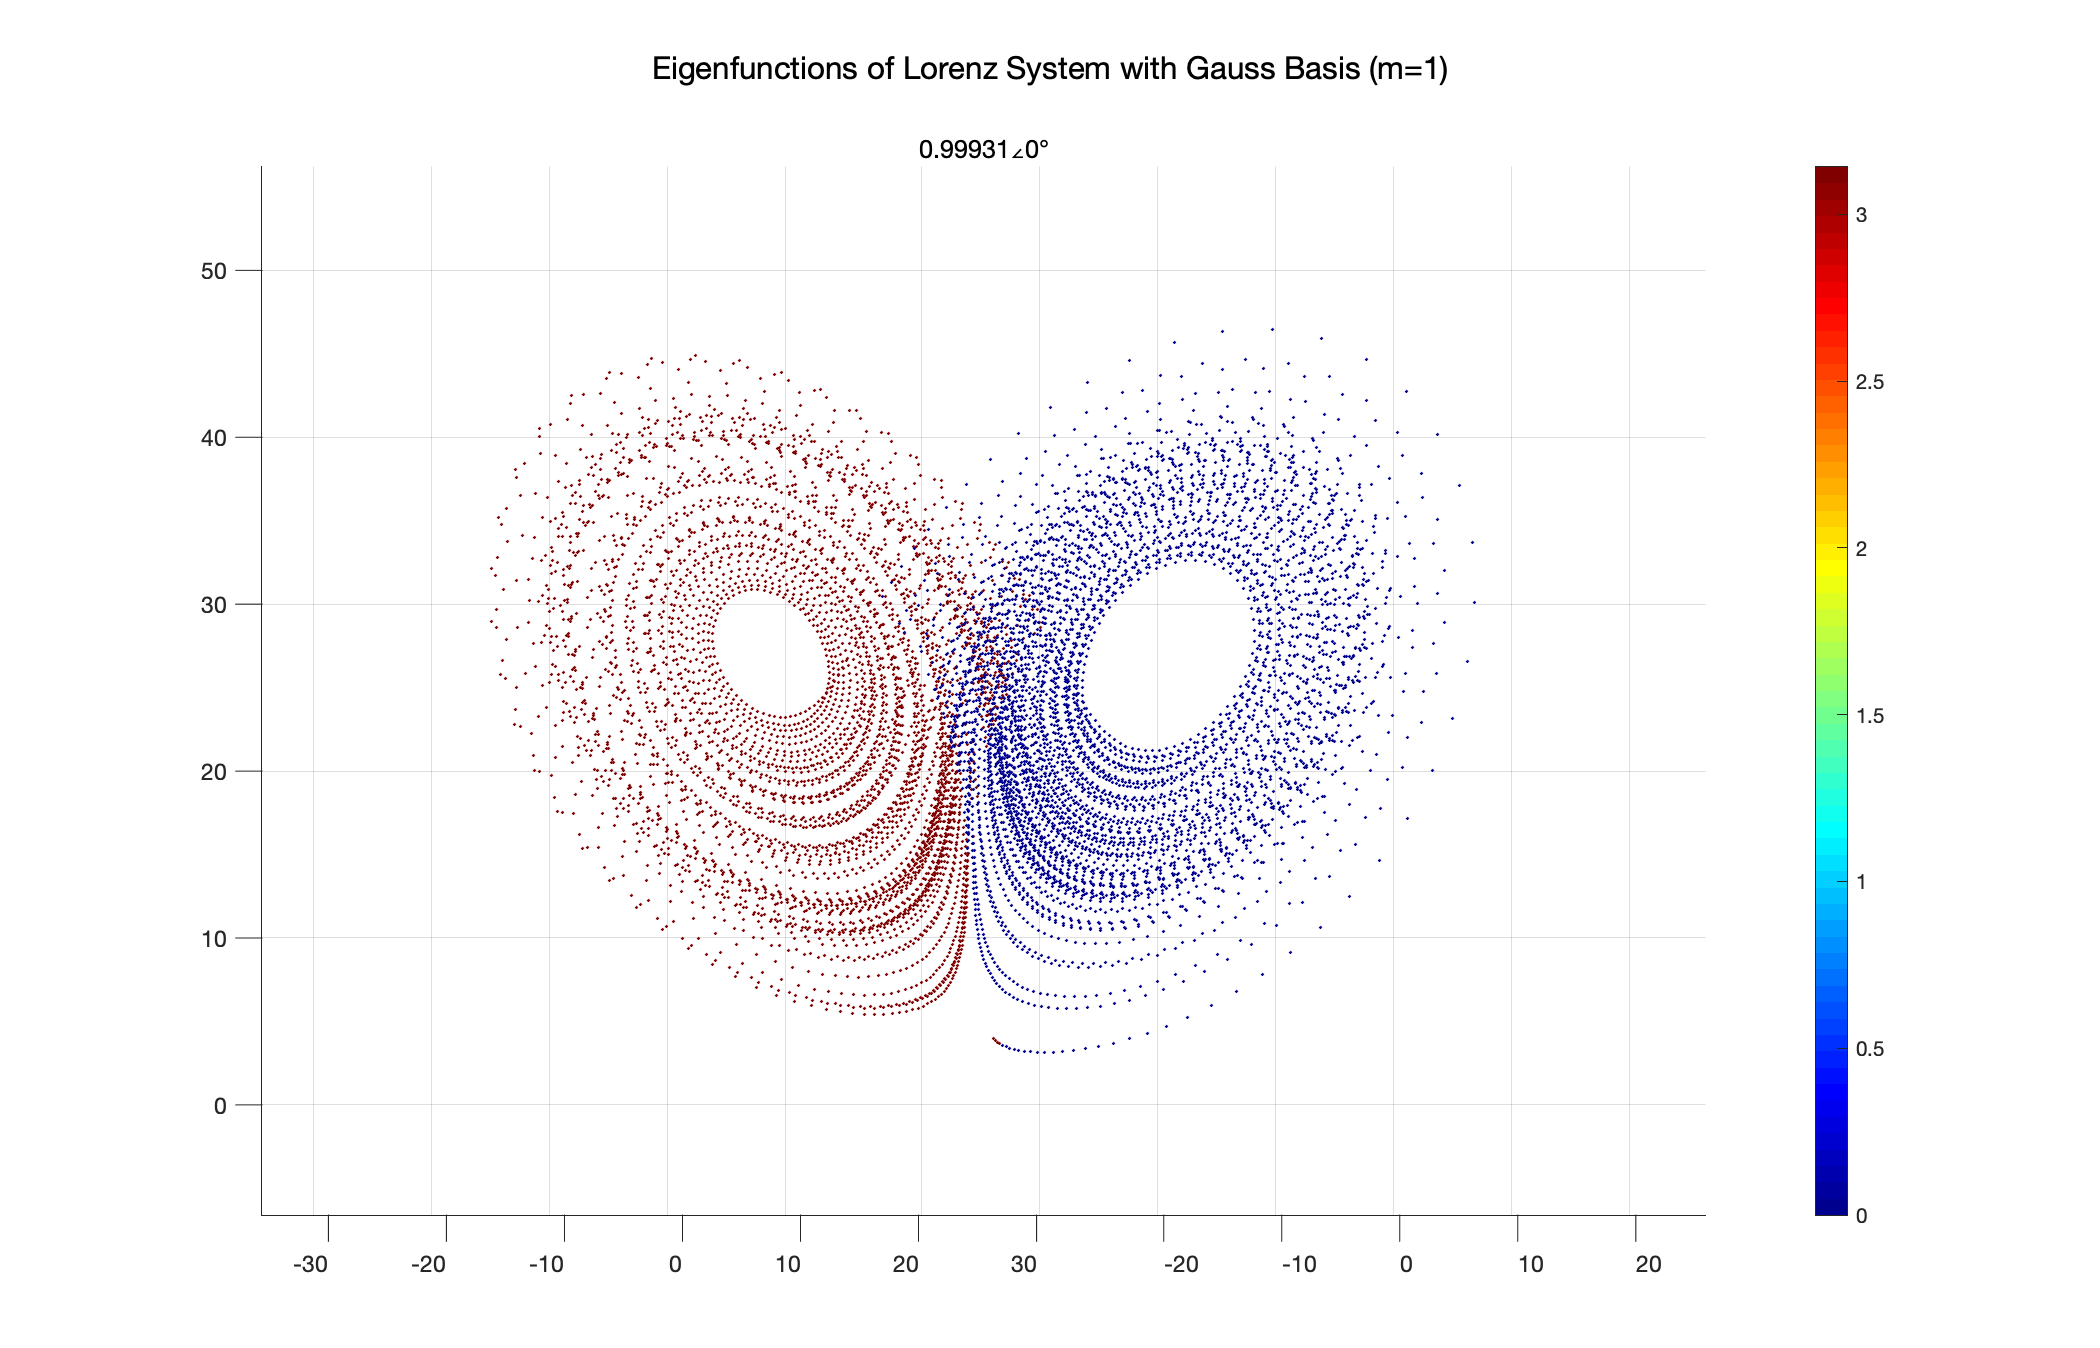
\includegraphics[scale=0.2]{lorenz/natural/multim/Lorenz_eigen_natural_multim_n10000m1dim1}}
    \subfloat[m=2]{
      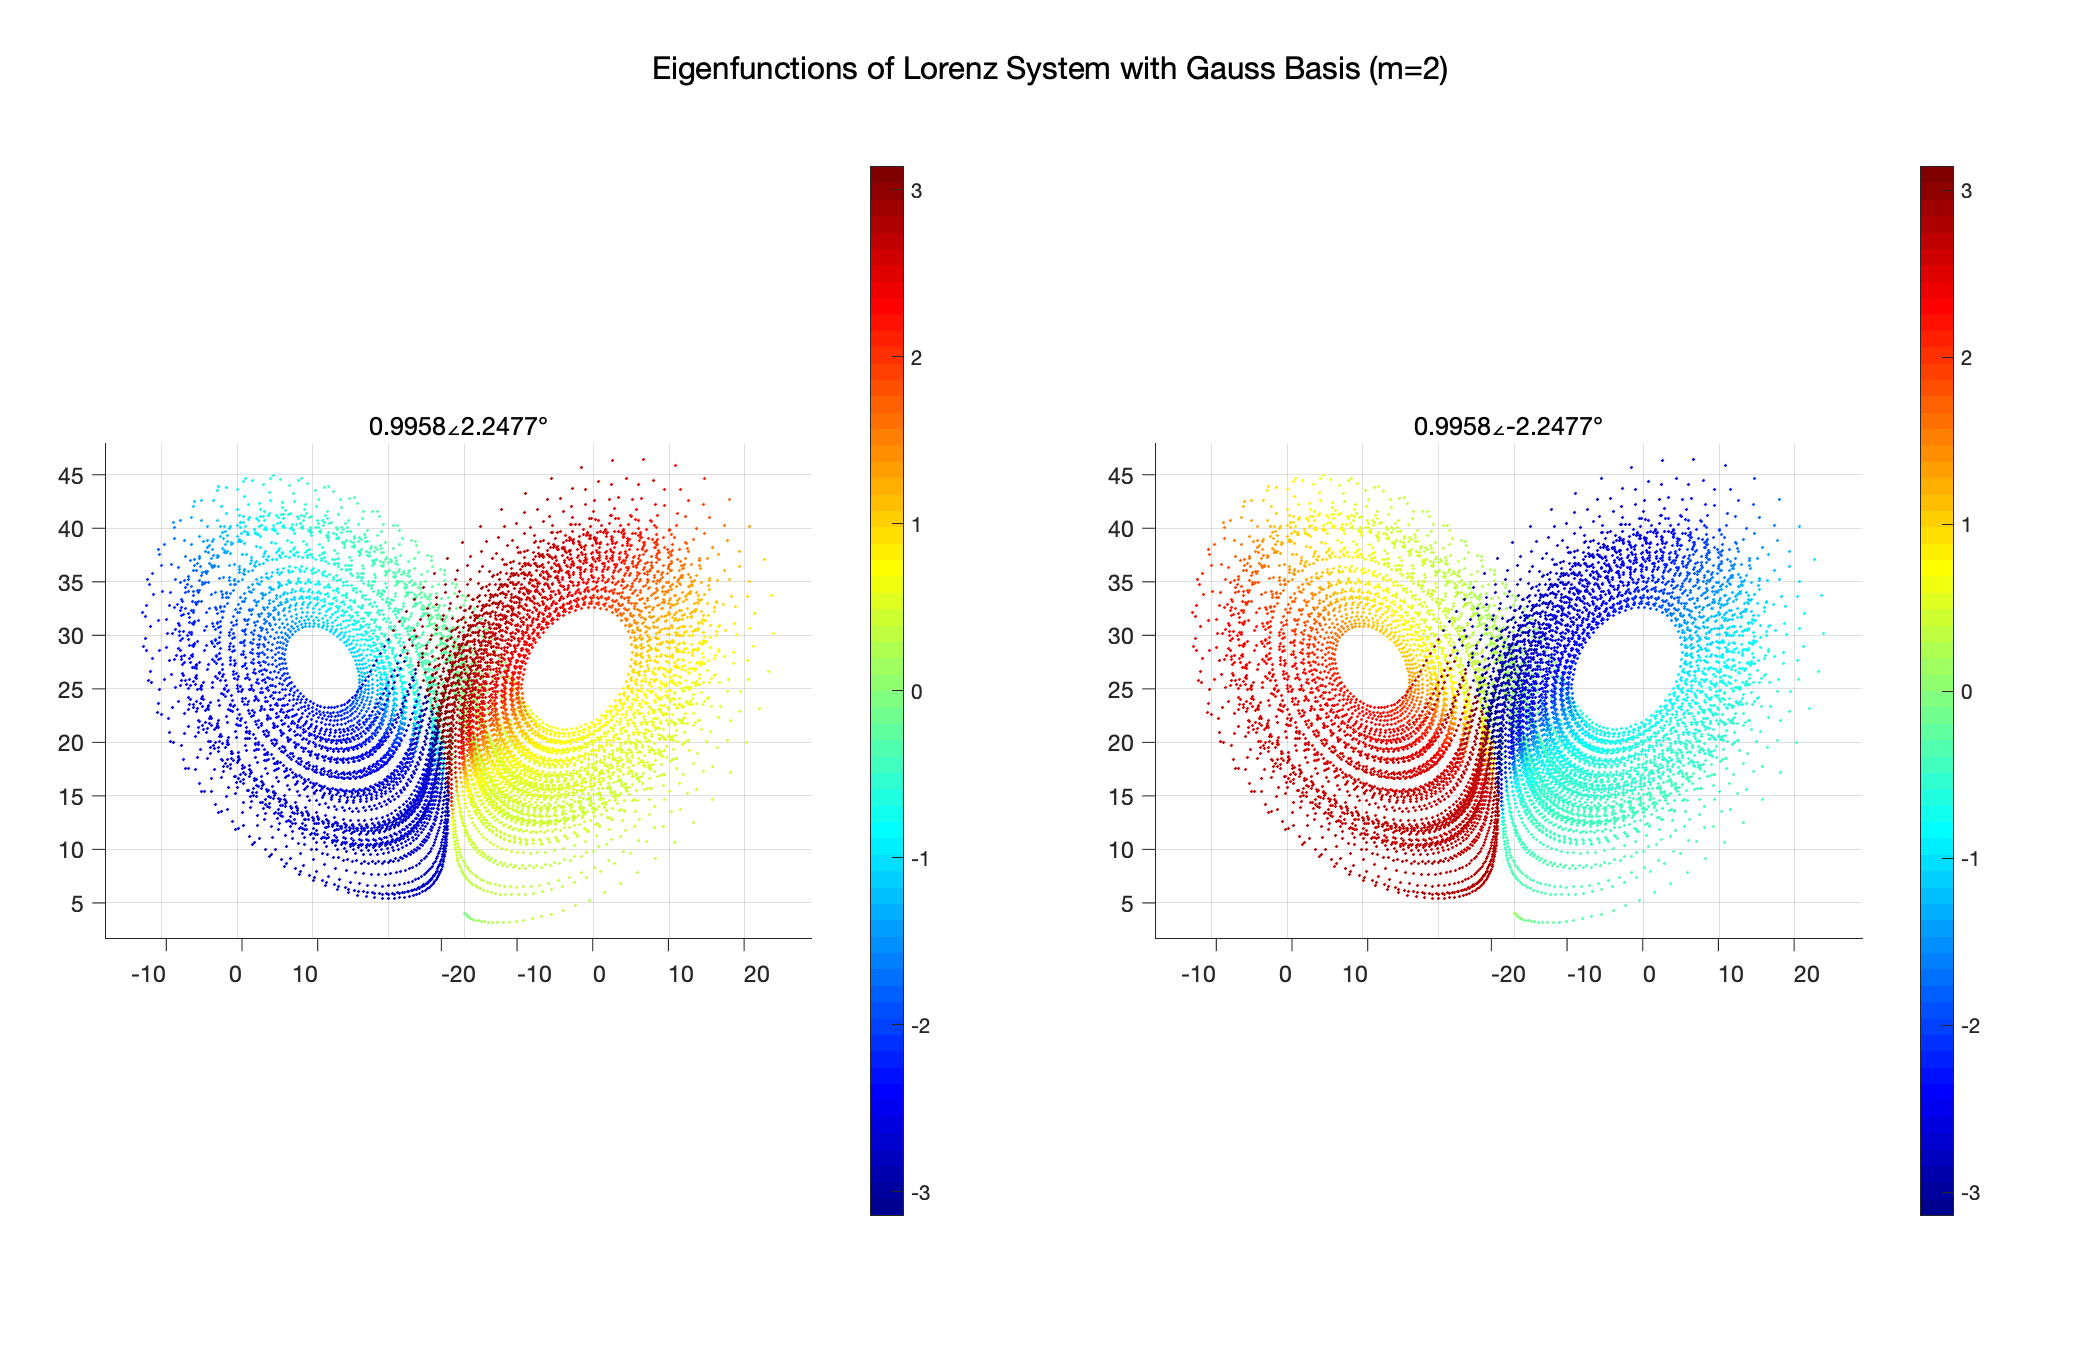
\includegraphics[scale=0.2]{lorenz/natural/multim/Lorenz_eigen_natural_multim_n10000m2dim1}}
    \\
    \subfloat[m=3]{
      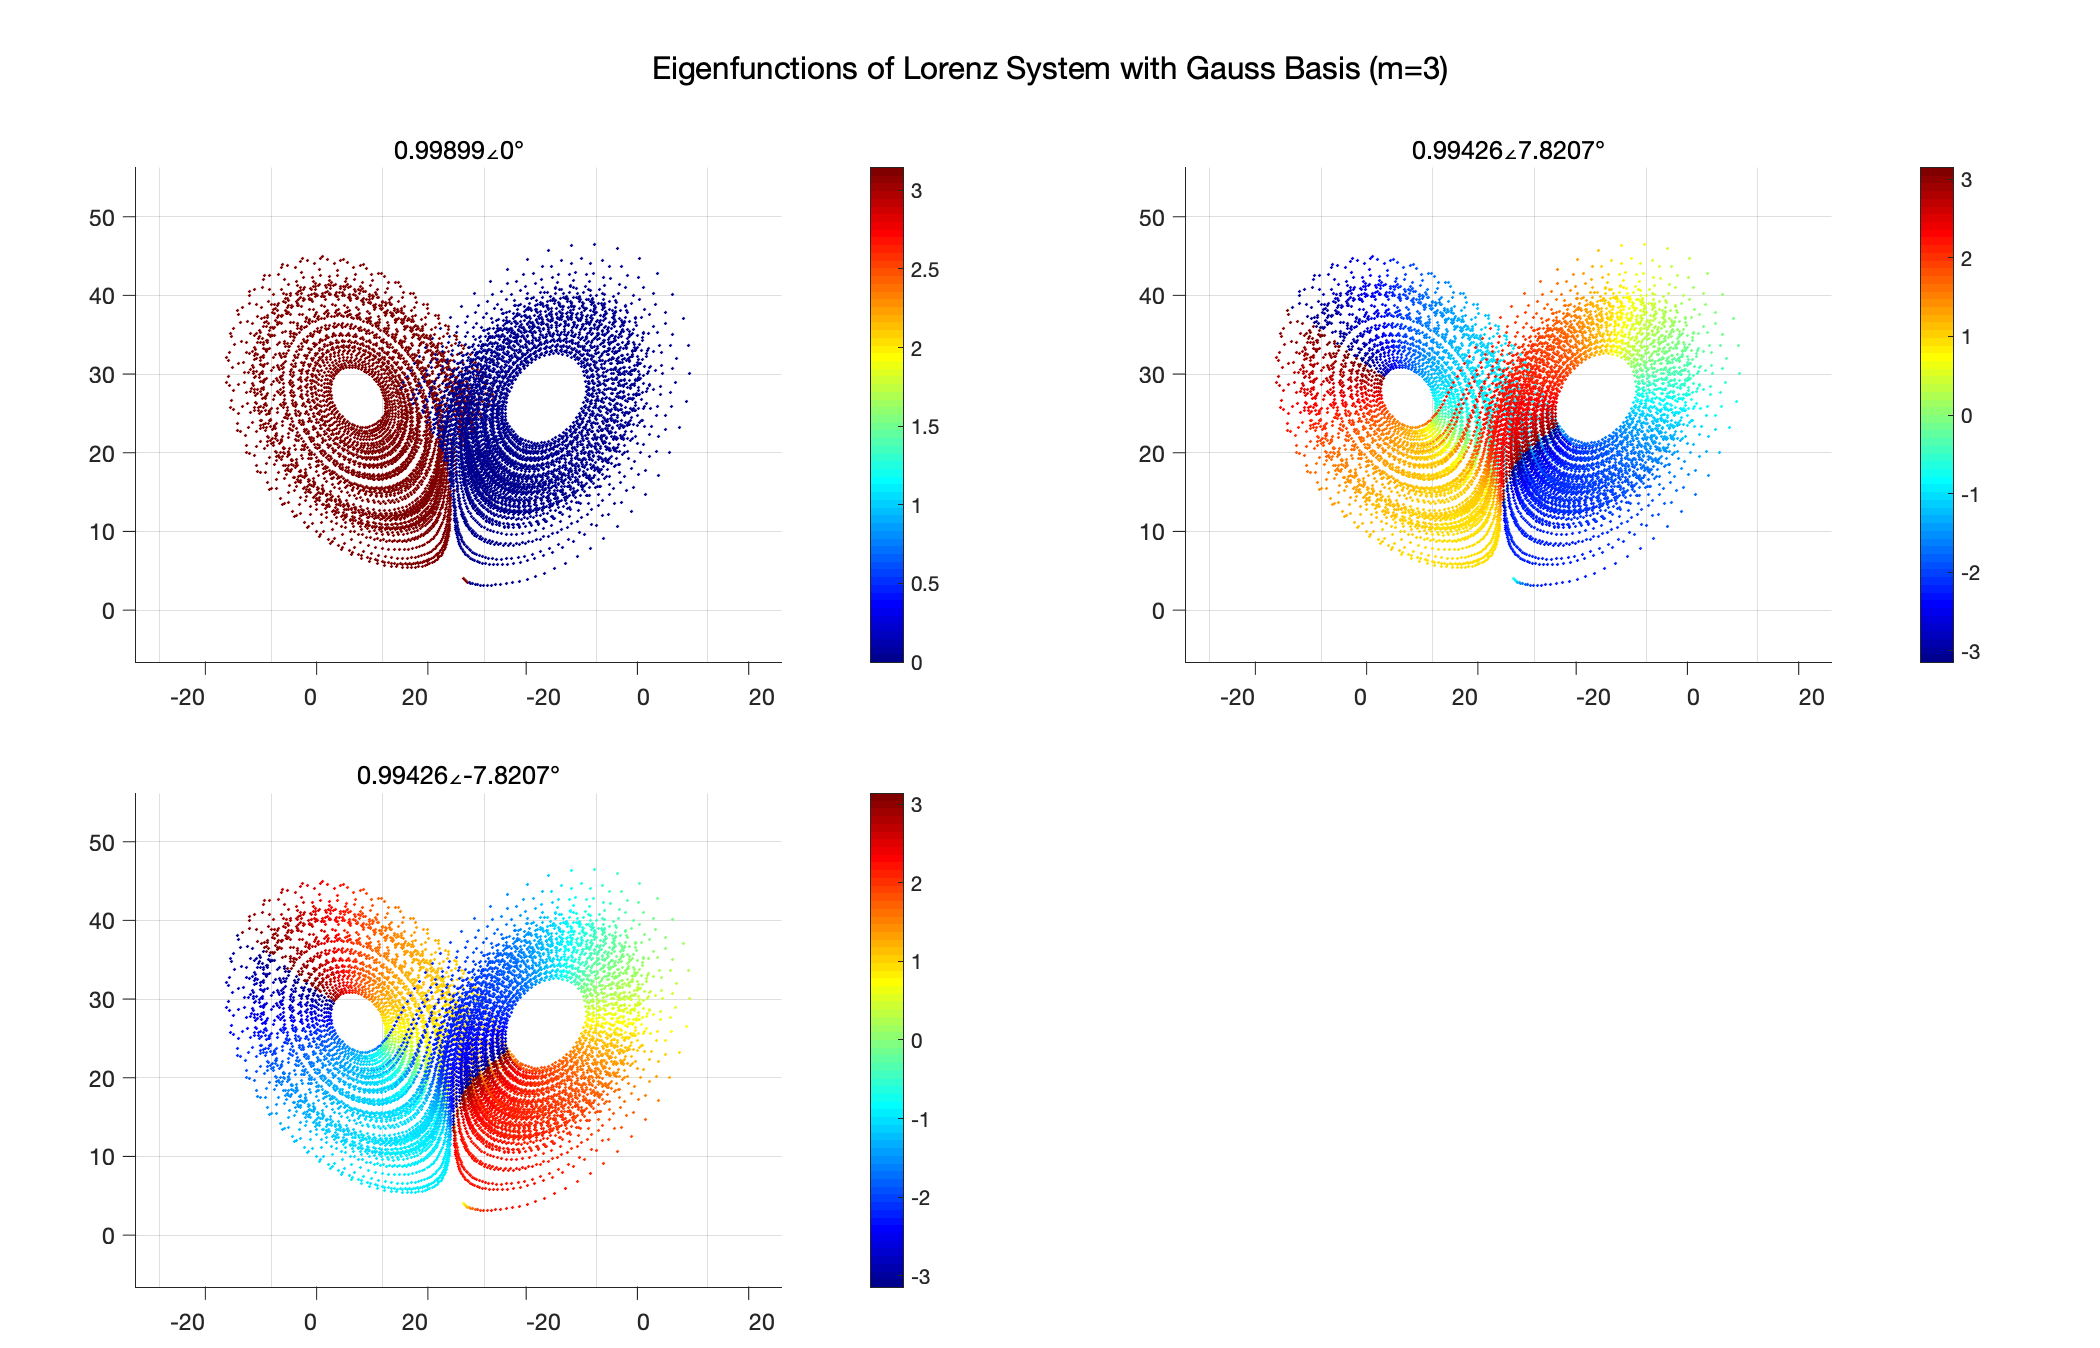
\includegraphics[scale=0.2]{lorenz/natural/multim/Lorenz_eigen_natural_multim_n10000m3dim1}}
    \subfloat[m=4]{
      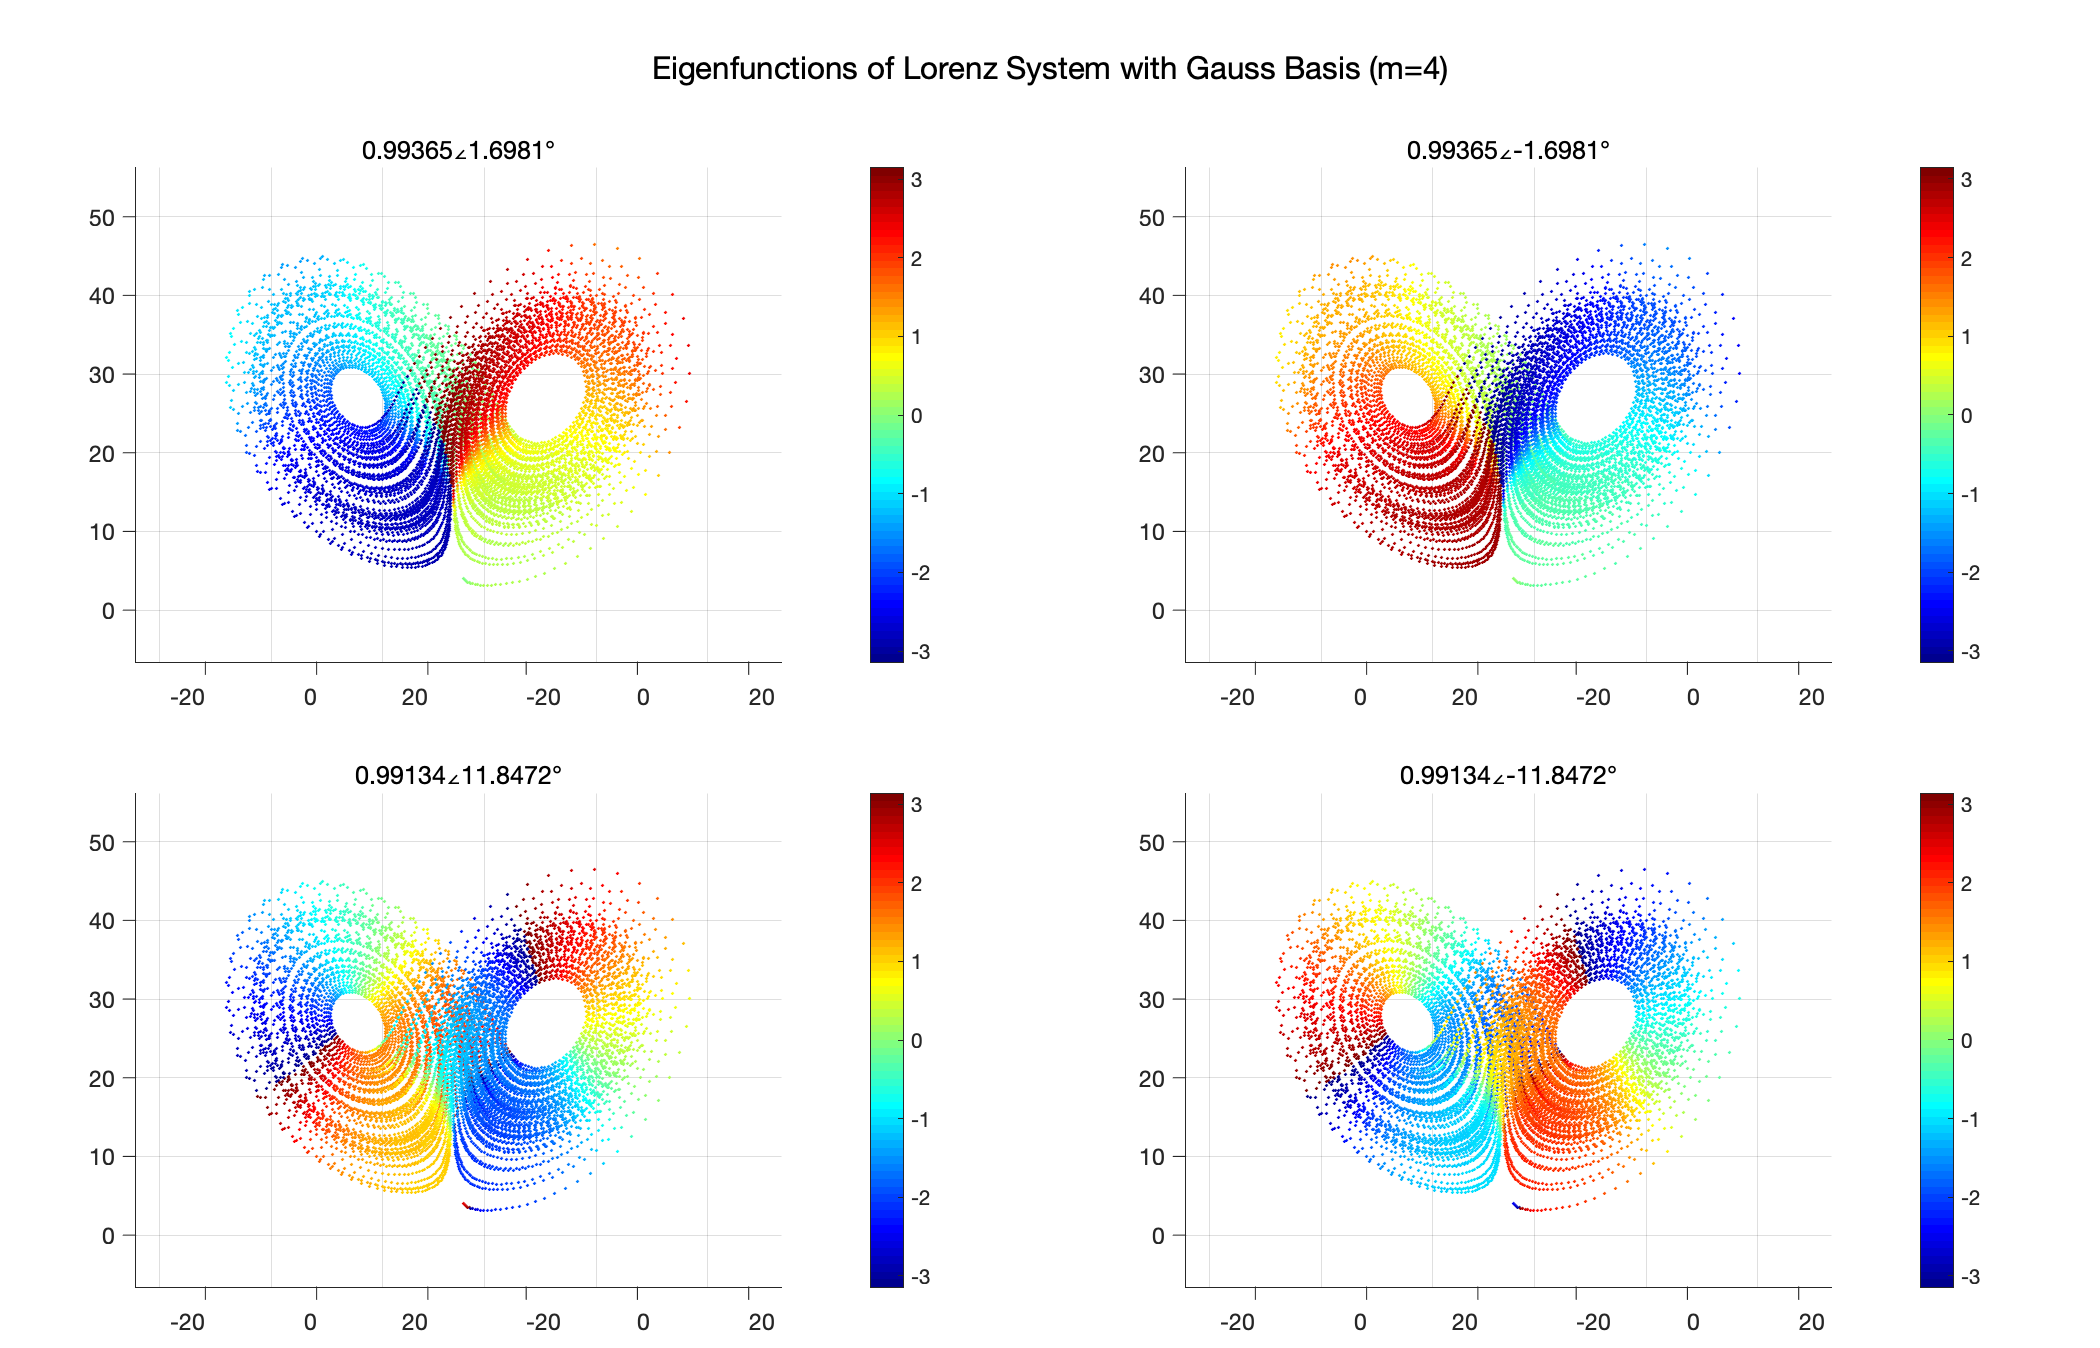
\includegraphics[scale=0.2]{lorenz/natural/multim/Lorenz_eigen_natural_multim_n10000m4dim1}}
    \\
    \subfloat[m=5]{
      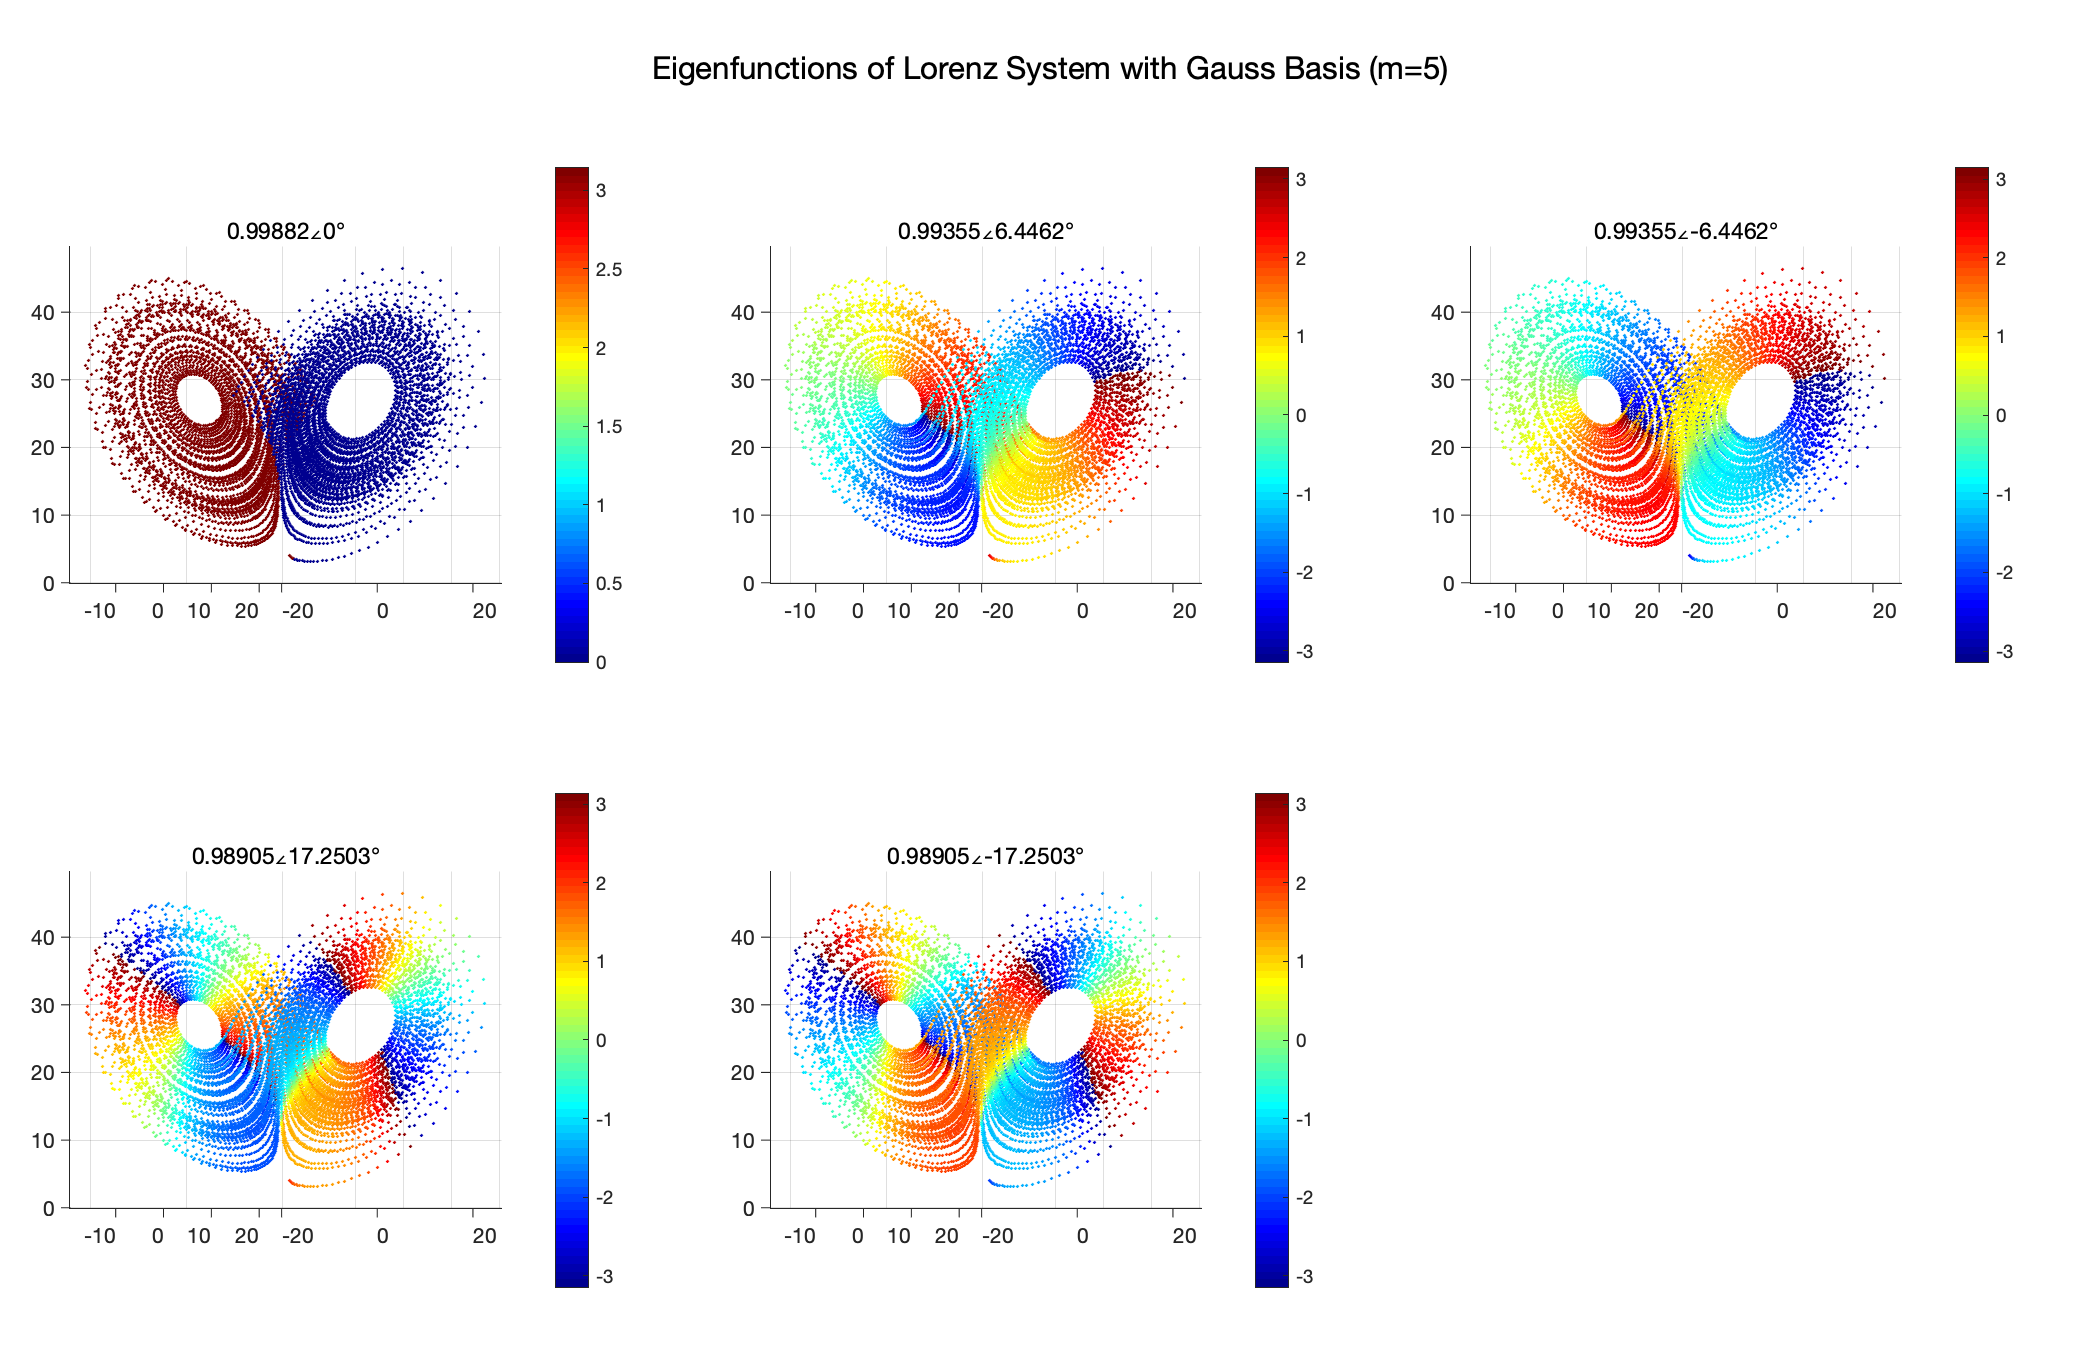
\includegraphics[scale=0.2]{lorenz/natural/multim/Lorenz_eigen_natural_multim_n10000m5dim1}}
    \subfloat[m=6]{
      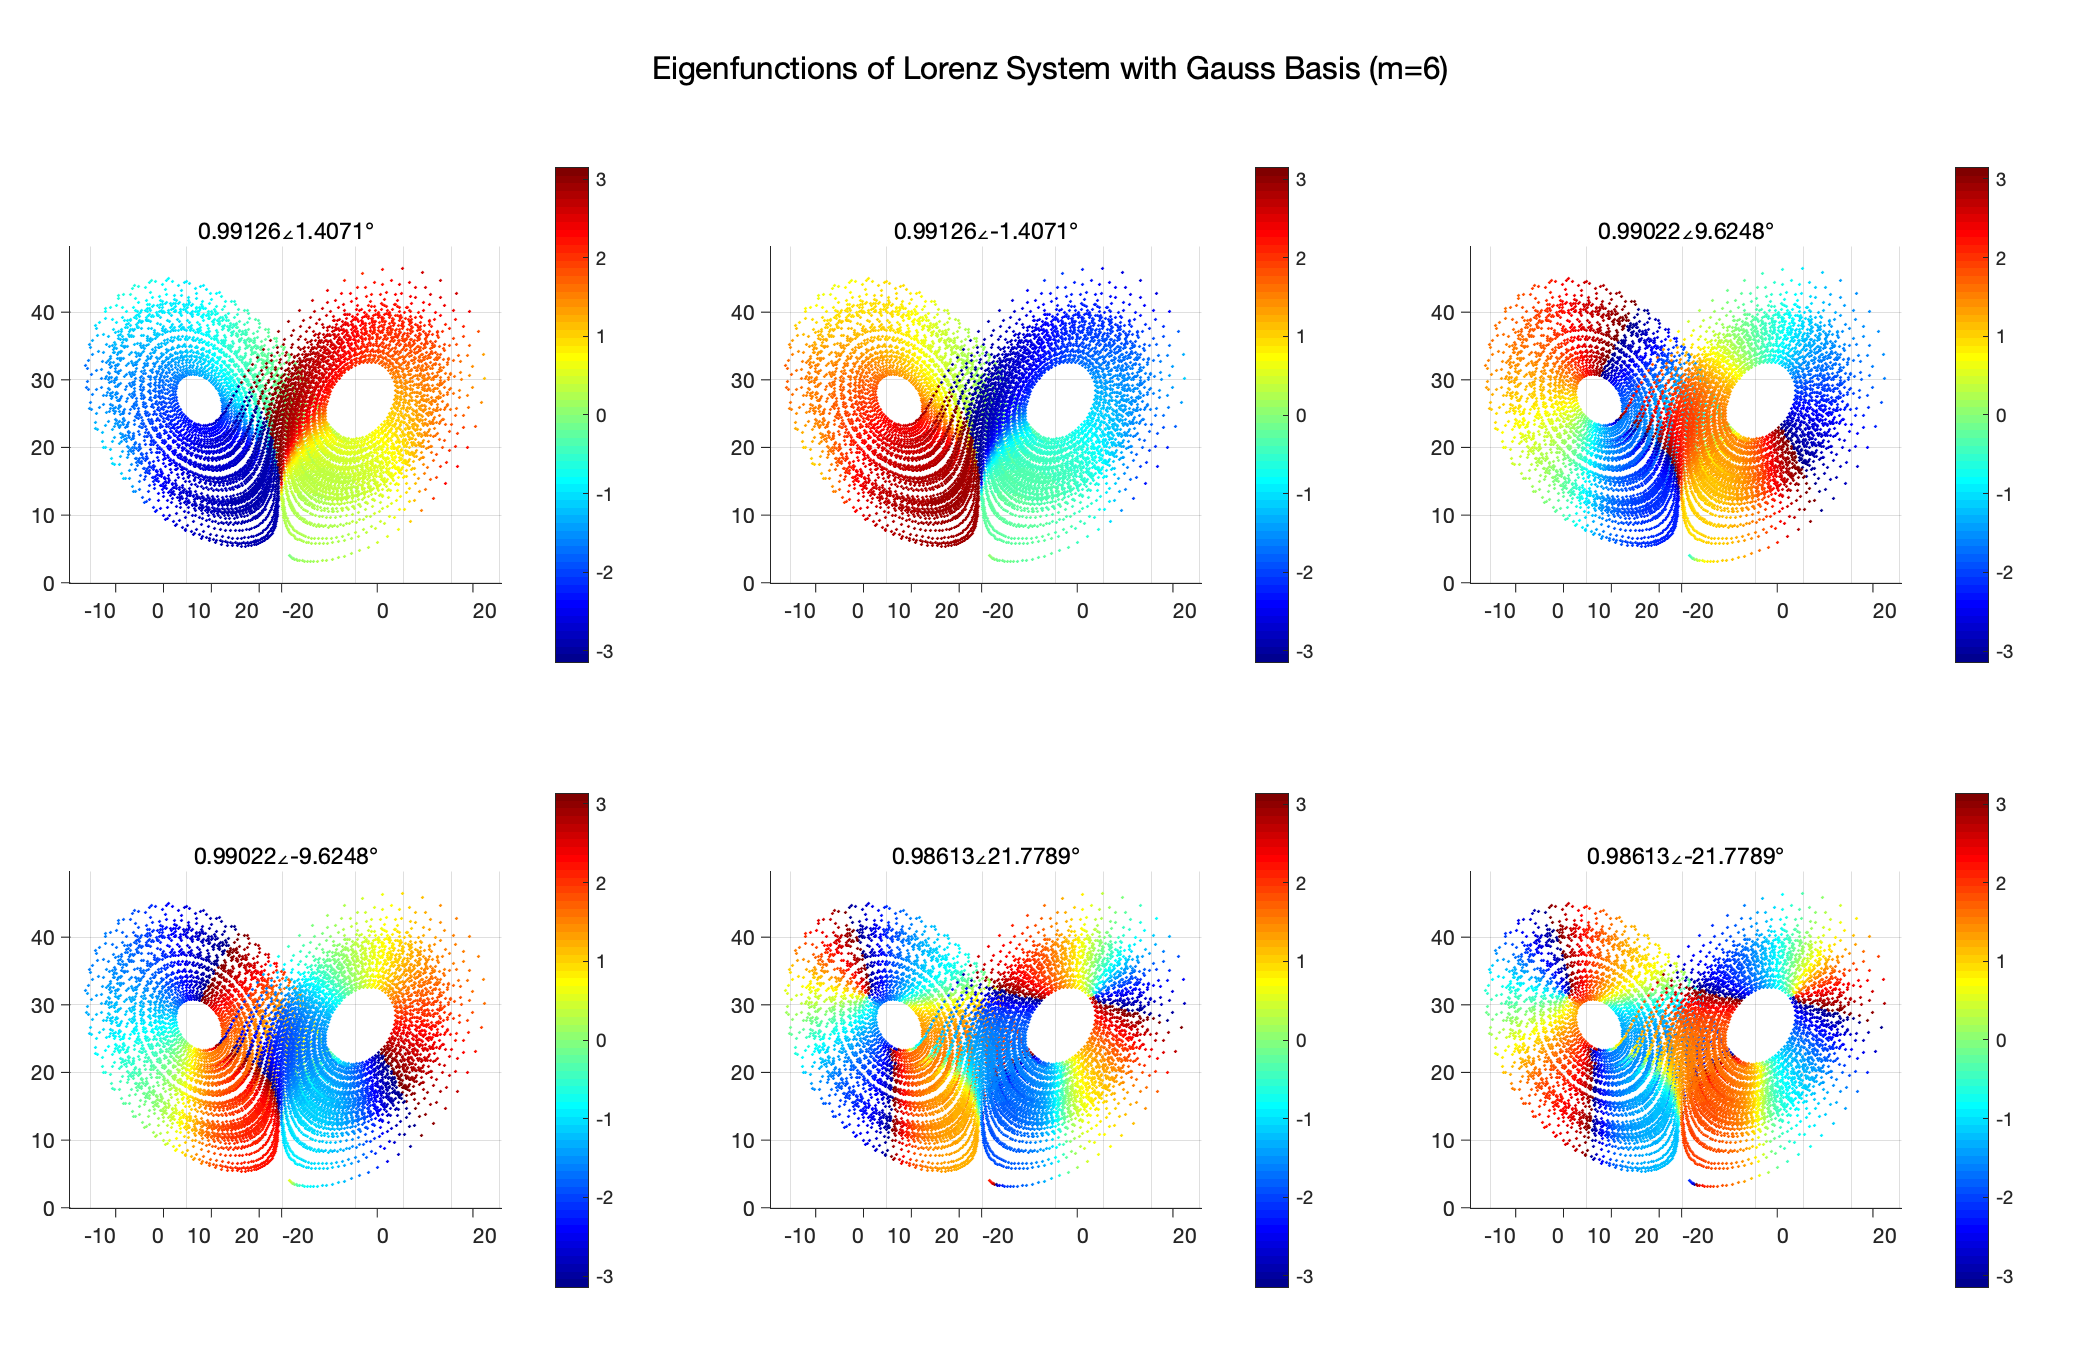
\includegraphics[scale=0.2]{lorenz/natural/multim/Lorenz_eigen_natural_multim_n10000m6dim1}}
    \\
    \subfloat[m=7]{
      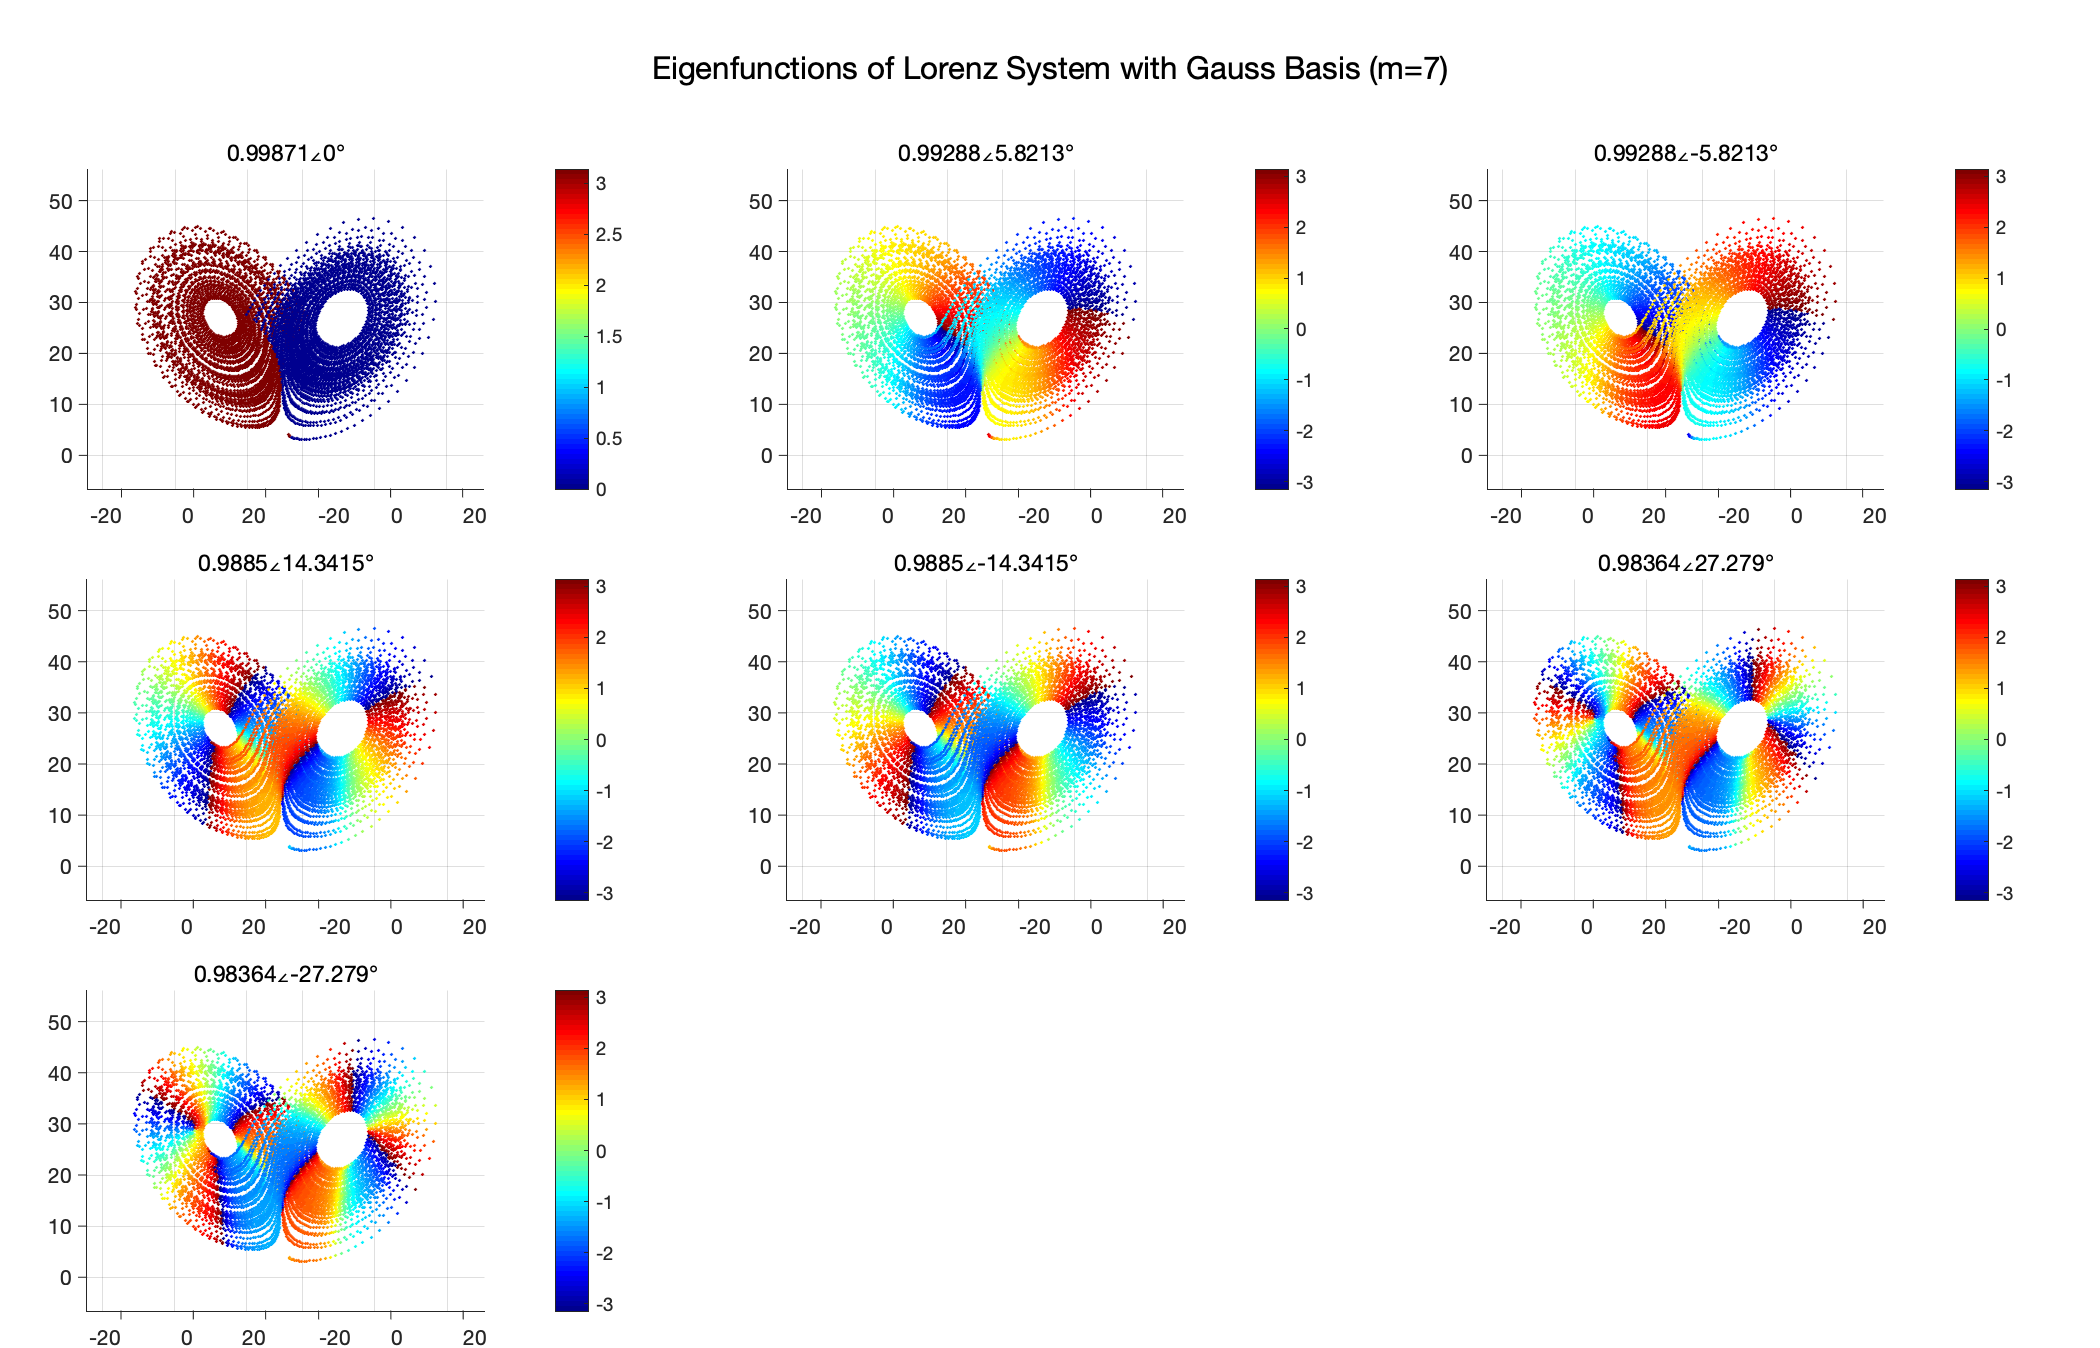
\includegraphics[scale=0.2]{lorenz/natural/multim/Lorenz_eigen_natural_multim_n10000m7dim1}}
    \subfloat[m=8]{
      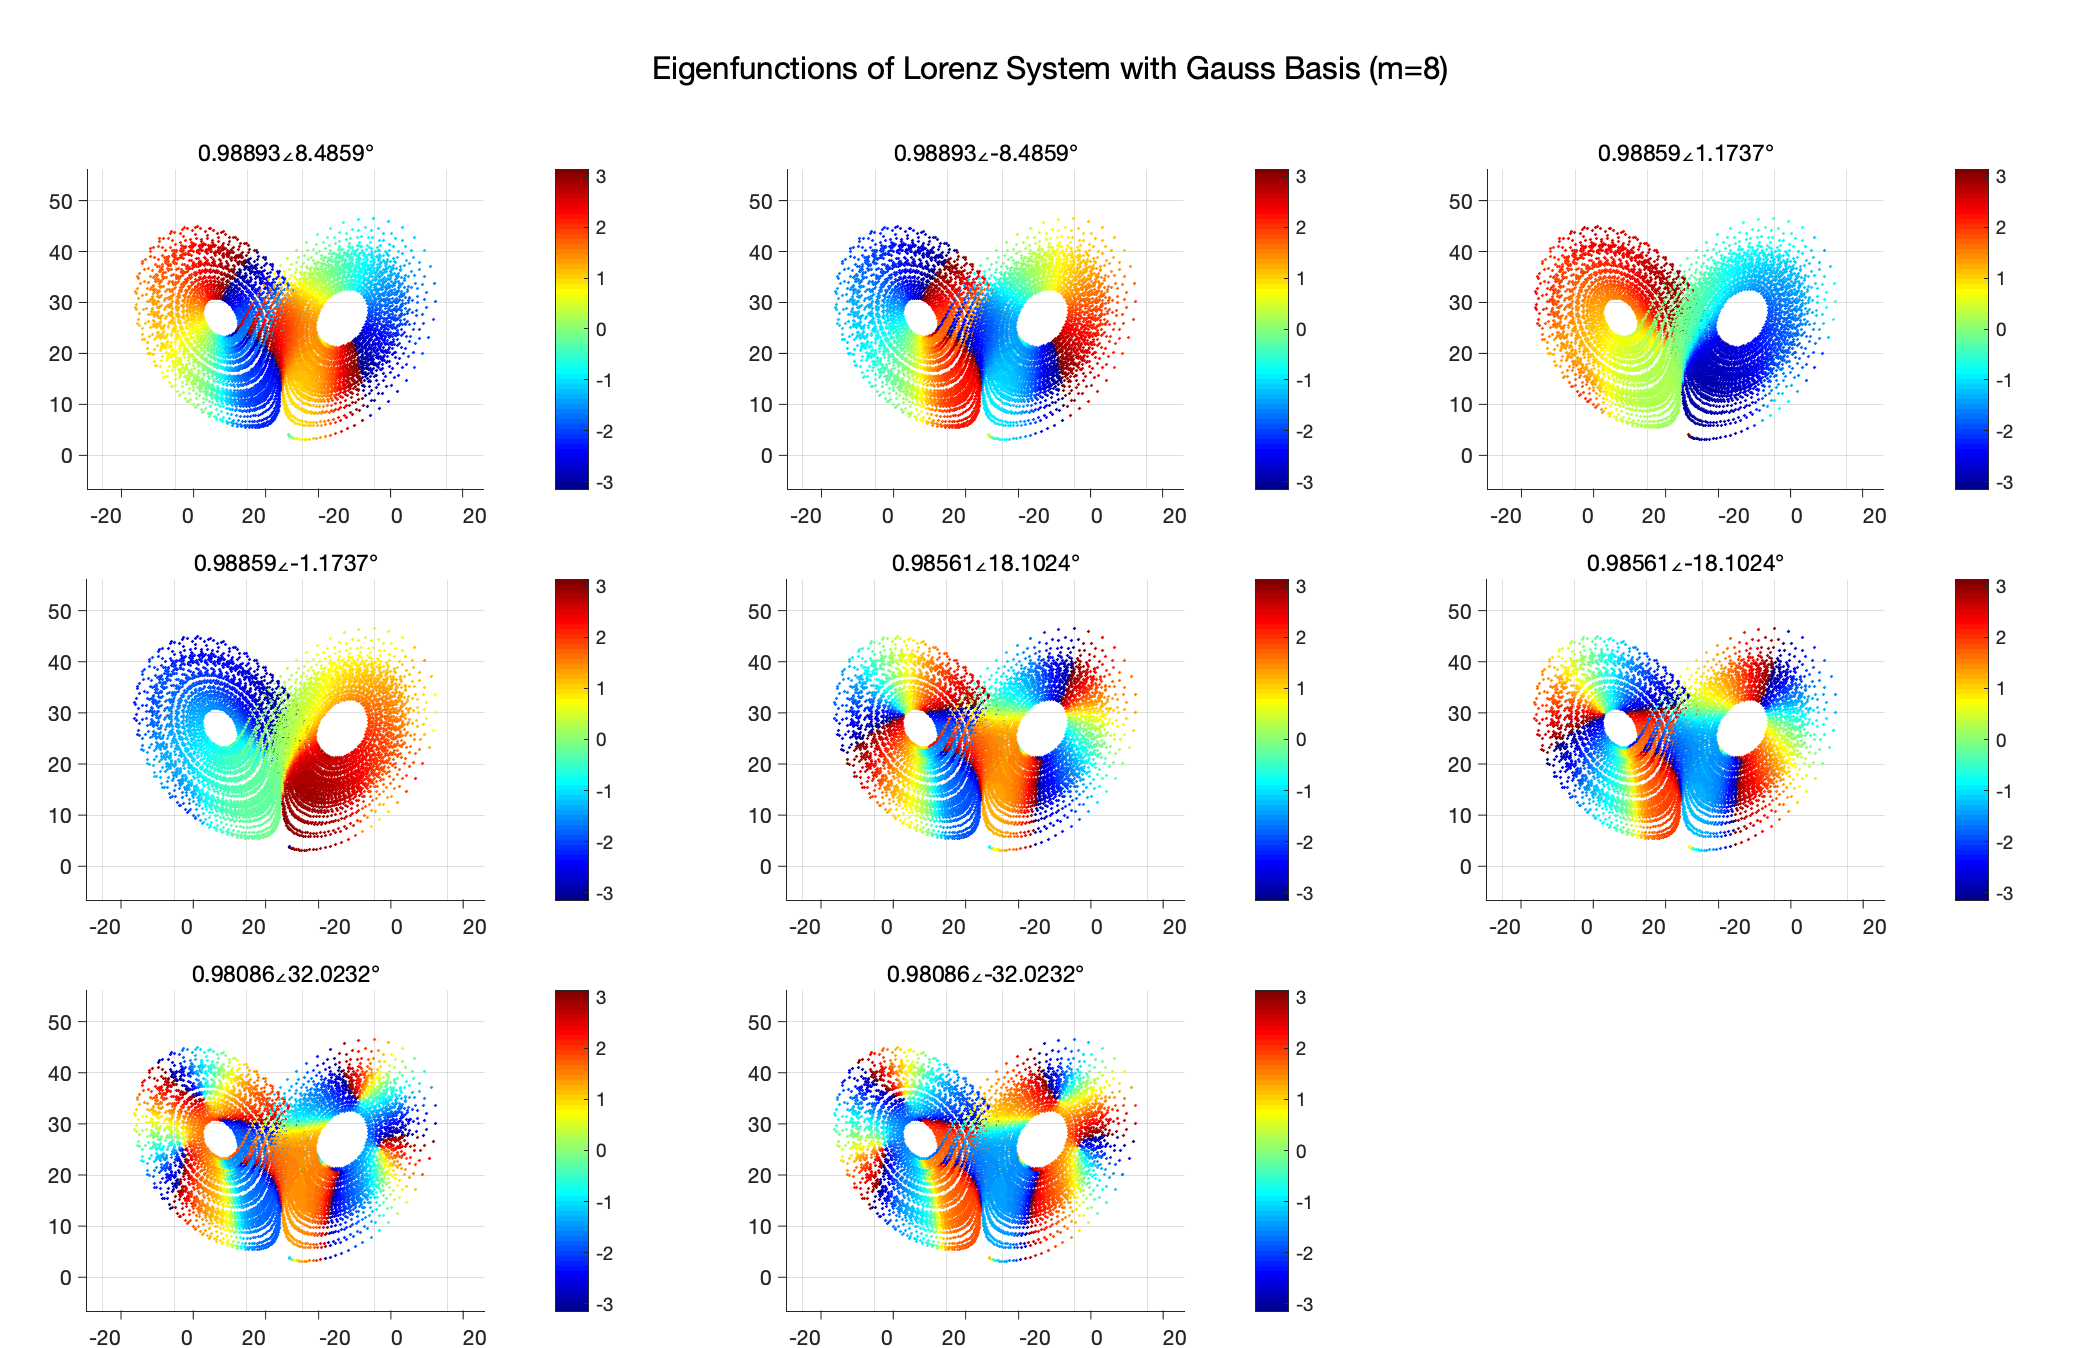
\includegraphics[scale=0.2]{lorenz/natural/multim/Lorenz_eigen_natural_multim_n10000m8dim1}}
    \\
    \caption{洛伦兹系统不同自然基函数数量下的real(x)本征函数($n=10000$)}
\end{figure}

\subsection{Koopman算符对洛伦兹系统的相空间划分}

\subsection{更多的讨论}
\subsubsection{噪声对Koopman算符的影响}

\subsection{小结}